\documentclass[14pt,a4paper]{extreport}
%\usepackage[utf8]{inputenc}
\usepackage{amsmath}
\usepackage{amsfonts}
\usepackage{amssymb}
\usepackage{mathptmx}
\usepackage{fullpage}
\usepackage{graphicx}


%\usepackage{setspace}  
%\setstretch{1.5}
%\usepackage{cite}
\usepackage[left=3.5cm,right=2cm,top=3cm,bottom=3.5cm]{geometry}


\author{Ngo Thanh Vu}
\title{EXPLORATION  OF  RIA  TECHNOLOGIES  AND  DEVELOPMENT  OF  A  WEB-BASED DIAGRAMMING TOOL}
%\linespread{1.5}
\begin{document}
\maketitle
\tableofcontents
\listoffigures
\listoftables


%Acknowledgement
\begin{titlepage}
\textbf{Acknowledgement}

I dedicate special gratefulness to my instructor, Dr.Do Lenh Hung Son for guiding and assisting me during the time i was working with him. I would like to thank all members in the Advanced Program of Computer Sciences including my classmates, seniors, professors, and all members in the Teaching Staff of Faculty of Information Technology and Academic Affairs. They play a very important part to the success of my thesis
\end{titlepage}

%Abstract
\begin{titlepage}
\textbf{Abstract}

Since 1999, when the term "Web 2.0" was introduced , which is associated with a richer web facilitating social media, user-generated content as well as interaction and collaboration, business applications have become increasingly web-oriented . While the web in its roots was limited to passive viewing of content created by others, it has moved towards an application platform for desktop-like applications within the last decade. Utilizing these advantages, in this thesis, I present a web application to design diagrams which can be considered as a Rich Internet Application (RIA) and Single Page Application (SPA). I also took a survey to explore and choose state of the art technologies which support to build such web application.I demonstrated by building an web application using the chosen technologies and integrating them . I also introducing about RIA and SPA as well as HTML5, CSS3, AngularJS (Javascript Framework), GoJS (Diagram Library), and other technologies i have been using for this application.

\end{titlepage}

\chapter{INTRODUCTION}

Nowadays Internet is increasing its popularity dramatically, people tend to work online with web browsers more than ever\cite{survey,Gvu,Center} . A survey in early 2010 \cite{Internet} showed that 74\% of American adults and 93\% of teenagers of age 12-17 use the Internet. More specific, email and search engines are the two most popular services that people do online\cite{Online}. Web browsers play a key role of being a door to link users to an enormous source of information: websites. Therefore, The popularity of web browser is premise for the emerging of web applications which uses web browser as a client. The ability to update and maintain web applications without distributing and installing software on potentially thousands of client computers is a key reason for their popularity, as is the inherent support for cross-platform compatibility\cite{WebApp}.
\\

Low-level JavaScript libraries like jQuery\footnote{http://jquery.com/}, Prototype\footnote{http://www.prototypejs.org/}, Underscore.js\footnote{http://documentcloud.github.com/underscore/}, etc., provide a convenient API for manipulating the Document Object Model (DOM) in a uniform way across different browser implementations. However no means to structure
the application code are provided, usually resulting in lots of DOM element selector and callback code\cite{Real}. This "spaghetti code of the 21st century" \cite{MT08} is reminiscent of software development in the 1970s and leads to poor maintainability of applications. That’s where web application frame-works come into play. Besides disburden developers from writing boilerplate code, frameworks can structure web applications enforcing the separation of different application parts. According to the Model-View-Controller design pattern \cite{Ree79b, Ree79a} frameworks usually separate user interface definition, application data, and business logic. Due to this modularization, frameworks support the fast development of applications and promote reuse as well as maintainability. As of today, several frameworks are available.
\\

The extensive usage of JavaScript in today 's web application induces the need for frameworks supporting faster development, better reusability and maintainability. As Model-View-Controller(MVC)is a well-known design pattern for server-side application development. It becomes even more important on client-side leading to several prevalent JavaScript MVC frameworks\cite{Real}. Therefore client-side JavaScript application frameworks will be of great importance for the development of futer web-based business application.
\\

The goal of this thesis is to analyze existing JavaScript frameworks with respect to various criteria such as structure, data-biding, Testing ability,ect. From the set of reviewed frameworks, one should be selected to design and implement a web application for edit and design interactive diagrams. Besides, JavaScript libraries supporting implementing interactive diagrams are also analyzed and selected. Other selected technologies for front-end development and database are also integrated. This thesis proposes a way of survey and select  as well as integrating state of the art technologies into a web application.In fact, there are web applications supporting edit interactive diagrams. I can list several famous name as follow. Big guy Google's draw.io\footnote{https://www.draw.io} has his own online diagram drawing application which use MxGraph\footnote{www.jgraph.com/mxgraph.html‎} and his own cloud storage to implement. Creately\footnote{http://http://creately.com/} provide an environment for designing diagrams with support of collaboration implemented with Adobe Flash\footnote{http://www.adobe.com/software/flash/about/}. Gliffy\footnote{http://www.gliffy.com/} and Lucidchart\footnote{https://www.lucidchart.com/} are also famous for their beautiful diagrams with collaboration support. Although the features demonstrated cannot be fancy and various as in those example application , This thesis is still an evidence of using JavaScript frameworks and cloud storage actually makes web application development less complex, less cumbersome and more maintainable than in the past.
\\
\\
\\

Concretely, This thesis contains
\begin{enumerate}
\item Conducting surveys about JavaScript frameworks and JavaScript Libraries which support implementing 
\item Exploration of selected technologies
\item Implementing a web application using selected technologies
\item Evaluation about the advantages that those technologies brought as well as some future works remain to be done
\end{enumerate}
This thesis consists of six chapters. Below is each chapter’s preview:
\begin{list}{•}{•}

\item  Chapter 1- Introduction. A brief introduction about the trend of web application as well as the importance JavaScript frameworks in web application development, their advantages and briefly describe what i do.

\item Chapter 2 - Technology survey. A brief introduction about RIA and SPA. I present surveys about JavaScript frameworks and JavaScript graph libraries, Their result and reasons why i choose them

\item Chapter 3 - Exploration of key technologies. Describe in details about AngularJS, GoJS, Mongolab, Angular Boostrap, Jquery, Semantic-UI, their advantages and reasons for choosing them.

\item Chapter 4 - Building application using selected technologies. Describe in details how i implemented using selected technologies.

\item Chapter 5 - Discussion \& conclusion. I present further disscussion about the web application, pros and cons, vision for future works. i end the thesis by summing up what i have done.

\end{list}

\chapter{TECHNOLOGY SURVEY }
	\textsl{In this chapter, the concept of Rich Internet Application(RIA) and Single Page Application(SPA) is introduced. Besides, I need to define some criteria based on what Javascript framework can bring. Consequently, i conducted surveys about JavaScript frameworks and JavaScript Graph libraries in order to support the web application development}
	\newpage 

	\section{RIA and SPA }
		\subsection{Introduction}
	

	
		Since 1990, when the first web browser prototype called "WorldWideWeb"\cite{BL12} was released by Tim Berners-Lee, the web has evolved from a simple document sharing system to a multimedia content distribution and application runtime environment. The major evolution step which is depicted in the picture below. At first, web pages were simple documents contain nothing but text and images.Users could navigate between different pages by hyperlinks.\\\\
		
		 At that time the capability of the web was limited. Due to emerging software development capabilities, the web was used increasingly as application platform in the second period. This is the time when the term \textbf{single-page application} also known as \textbf{single-page interface (SPI)} appears. It is a web application or web site that fits on a single web page with the goal of providing a more fluid user experience akin to a desktop application.
		 
		\begin{figure}[ht]
		 \begin{center}
			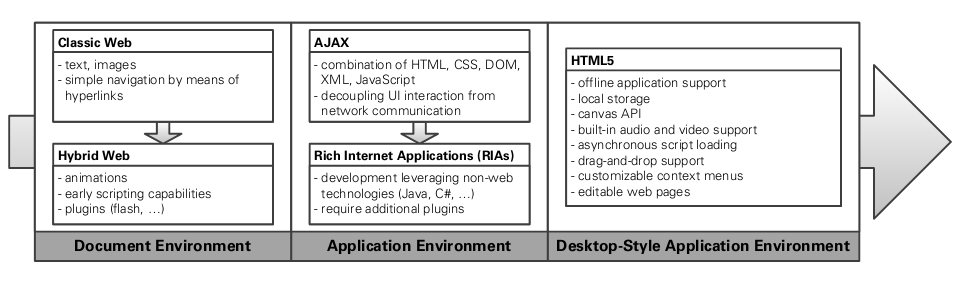
\includegraphics[scale=0.5]{WebEvolve.png}
			\caption{Major evolution steps of the Web\cite{TM11}}
		\end{center}
		\end{figure}
		\textbf{Asynchronous JavaScript and XML (AJAX)}, introduced by Jesse James Garret in 2005\cite{Gar05} ,changed the primary interaction model of the web and therefore increased its use as an application environment. However, the browser at this time was not supplied enough comprehensive sets of \textbf{API} and complex graphic capabilities.To provide such sets of APIs which were similar to the desktop application, \textbf{RIA} is introduced. It is a Web application that has many of the characteristics of desktop application software, Users generally need to install a software framework using the computer's operating system before launching the application, which typically downloads, updates, verifies and executes the RIA\cite{RIA} .Examples for RIA platforms are Adobe Flash,Java FX and Microsoft Silverlight.
		
		
		\subsection{The current approaches}
		
			\subsubsection{JavaScript}
		
		 Currently JavaScript is the predominant implementation technique for plug-in free applications in the web. JavaScript applications can be built by means of pure JavaScript, leveraging low-level libraries like jQuery or high-level frameworks like Knockout.js. Since applications built by means of JavaScript use standardized web technologies, they do not require a dedicated plug-in
as runtime environment.
			\subsubsection{Non-JavaScript}
		
			Non JavaScript, but plug-in based applications require the installation of additional browser plug-ins serving as runtime aaenvironment. Example technologies belonging to this category are Adobe Flash , Java FX and Microsoft Silverlight.Some non JavaScript, but plug-in free implementation techniques are available too. Some of them enable the developer to write the application’s code in a language abstracting from concrete web technologies like HTML, CSS, etc. Two example technologies are Google Web Toolkit enabling web application development in Java, and CoffeeScript.
		
	\section{JavaScript Framework Selection}
		\subsection{Overviews of some JavaScript frameworks}
		\subsubsection{JavaScript Library view}
			we may define this group consists of the JavaScript framework which slots into your existing architecture and add specific functionality. Example to this kind are \textbf{Knockout.js, JQuery, JQueryUI}.JavaScript widget libraries such as \textbf{Ext JS , DHTMLX , Dojo Toolkit} were developed, allowing for developers to concentrate more upon more distinctive applications of Ajax.
		\subsubsection{JavaScript Framework view}
			This kind of framework gives you an architecture (file structure, etc.) that you are meant to follow and, if you do, are intended to handle all common requirements. Some example are \textbf{Ember.js , Angular.js , YUI, Backbone.js}
		
		\subsection{Framework Selection Characteristics}
		These are some criteria for choosing the framework
		\begin{itemize}
			\item The license under which the framework is released
			\item The size of the framework
			\item Community: the number of users or posts in the forum they use or on GitHub( Jan 2013) indicating the community support, as well as the website of the framework usually providing tutorials and a more or less comprehensive documentation.
			\item Programming language
			\item Js include indicates whether we need to include a js file into the website or not
			\item Basic UI component support: indicates that whether the framework provides their own basic component like text field, check box, combo box, form, date picker, ...
			\item Advanced UI widget library indicates that whether the framework support advanced components like grid view, tree, auto-complete, 
			
		\end{itemize}
		\subsection{Survey of Existing Frameworks}
		\subsubsection{Google Web Toolkit(GWT)}
			\begin{itemize}
				\item Overview: \textbf{GWT} provides an open source set of tools that allows web developers to create and maintain complex JavaScript front-end applications in Java. Besides,it supports writing both the client-side code and the server-side code in Java
				\item Pros: 
					\begin{itemize}
						\item supports ability to debug
						\item Strong community
						\item good documents,demos, samples
						\item supports lots of features
						\item No JavaScript syntax errors
						\item it's good for those who had java background and doesn't really appreciate the power of JavaScript (for both GWT and Vaadin
					\end{itemize}
				\item Cons:
					\begin{itemize}
						\item kind of a little too few stunning UI components comparing with Vaadin
						\item don't see much demo or support about drag drop
					\end{itemize}
			\end{itemize}
			\begin{figure}
				\begin{center}
					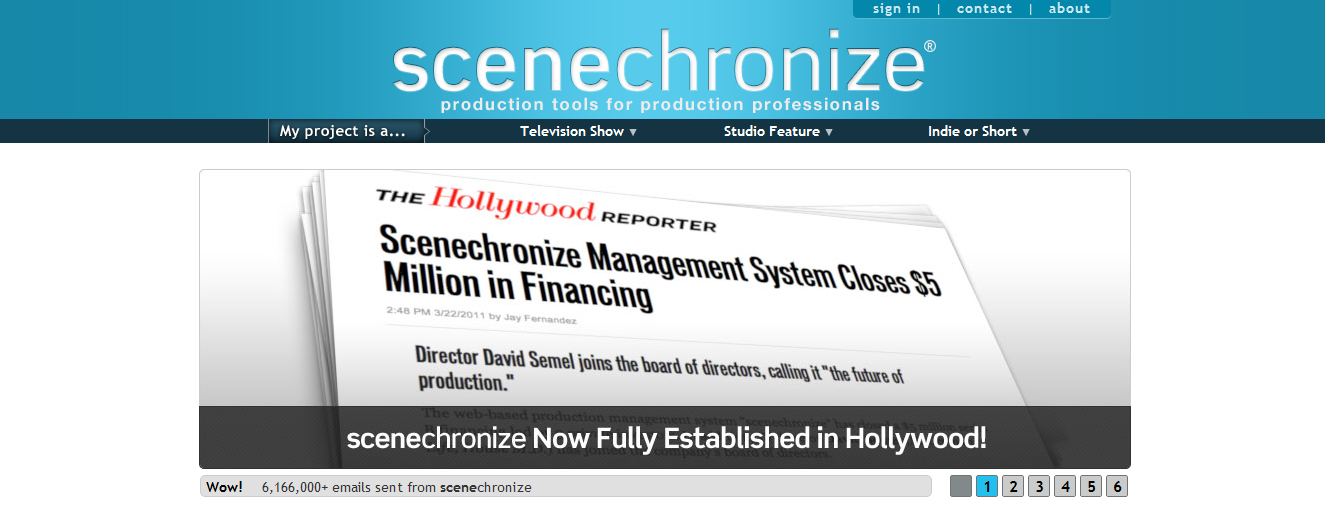
\includegraphics[scale=0.5]{GWT.png}
					\caption{ An example created by GWT}
				\end{center}
 			\end{figure}
			
		\subsubsection{Vaadin}
			\begin{itemize}
			\item Overview: features a server-side architecture and client-side is built on top of GWT.
				\item Pros: 
					\begin{itemize}
						\item Wide variety of UI components
						\item Drag and Drop for Tables, Panels and Trees components have real nice demos and tutorial
						\item Simple to learn, it has a book, a road map, a forum
						\item With Vaadin, you can build a nice app with almost a half of lines of code and still the application seems more complete compare with GWT
						
					\end{itemize}
				\item Cons:
					\begin{itemize}
						\item for advanced customization you'll need to write more in CSS, HTML, JavaScript
						\item Client side is not extensible and very chaotic
						\item html files is really heavy and takes long render time due to lots of components are added
						
					\end{itemize}
			\end{itemize}
			\begin{figure}
				\begin{center}
					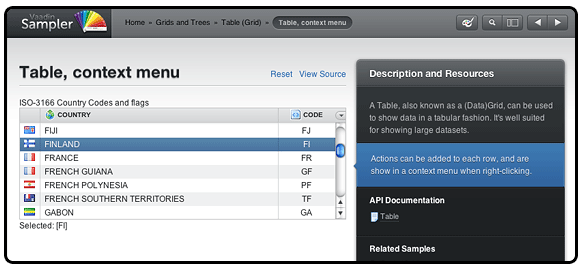
\includegraphics[scale=1.1]{Vaadin.png}
					\caption{An example created by Vaadin}
				\end{center}
			\end{figure}
		\subsubsection{SproutCore}
			\begin{itemize}
			\item Overview: an open-source framework for building blazingly fast, innovative user experiences on the web supported by Apple. It is also one of the largest frameworks.
				\item Pros: 
					\begin{itemize}
						\item MIT license
						\item Bindings support.
						\item Solid community. 
						\item Tons of features.
					
					\end{itemize}
				\item Cons:
					\begin{itemize}
						\item Overly prescriptive. 
						\item Hard to decouple from unneeded features.
						\item Forces a native-like paradigm
						
					\end{itemize}
			\end{itemize}
			\begin{figure}
				\begin{center}
				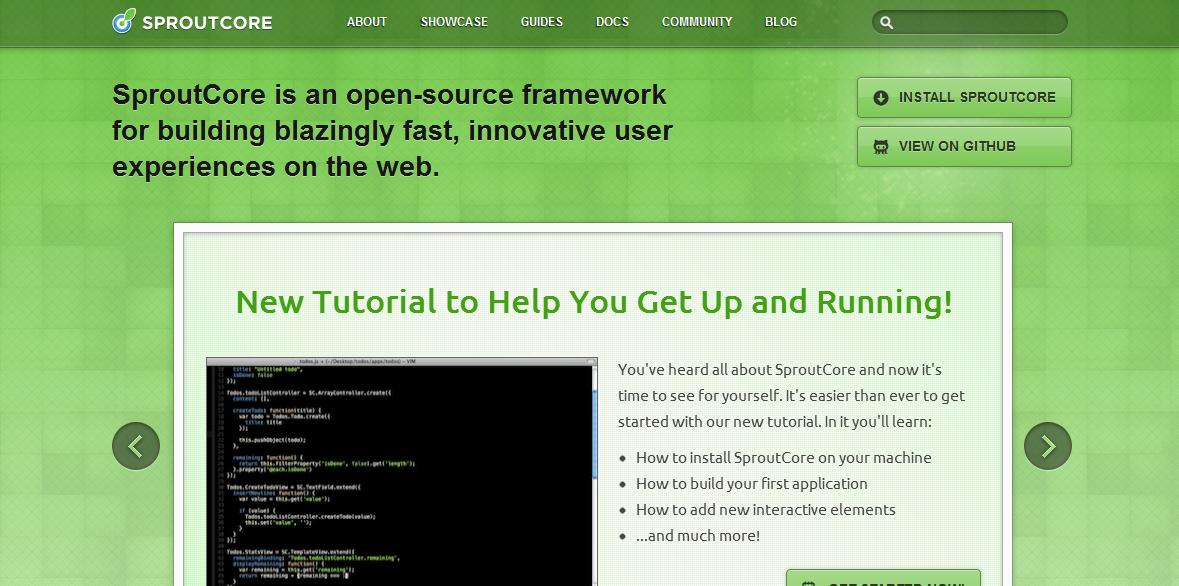
\includegraphics[scale=0.5]{Sproutcore.png}
				\caption{An example created by SproutCore}
				\end{center}
			
			\end{figure}

		\subsubsection{Dojo}
			\begin{itemize}
				\item Overview: DOJO is one of the leading JavaScript framework.
				\item Pros: 
					\begin{itemize}
						\item documents and tutorials in details
						\item  has all the components you would most likely use
					\end{itemize}
				\item Cons:
					\begin{itemize}
						\item API stability
						\item Demo is not very clear and scatter
						\item Many have commented that Dojo seems difficult to learn and get started with
			
					\end{itemize}
			\end{itemize}
			
			\begin{figure}
				\begin{center}
				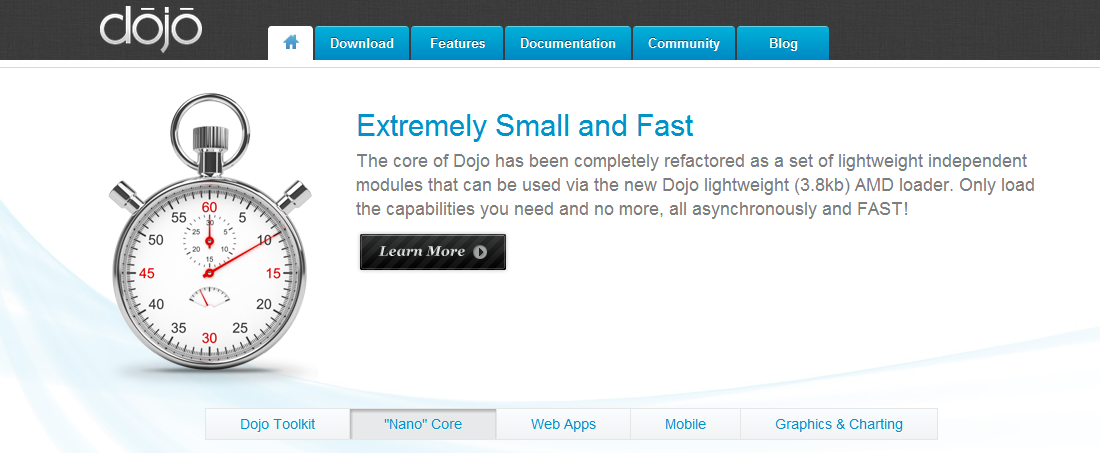
\includegraphics[scale=0.6]{Dojo.png}
				 \caption{An example created by Dojo}
				\end{center}			
			\end{figure}

		\subsubsection{JavaScriptMVC}
			\begin{itemize}
				\item Overview: an open-source framework containing the best ideas in jQuery development,a collection of the best practices and tools for building JavaScript applications. Built on top of jQuery"
				\item Pros: 
					\begin{itemize}
						\item using Controllers can make a clean, tight code that is easy to find
						\item is very lightweight, it's jQuery based
						
					\end{itemize}
				\item Cons:
					\begin{itemize}
						\item No preset UI layer implementations
						
					\end{itemize}
			\end{itemize}
			\begin{center}
			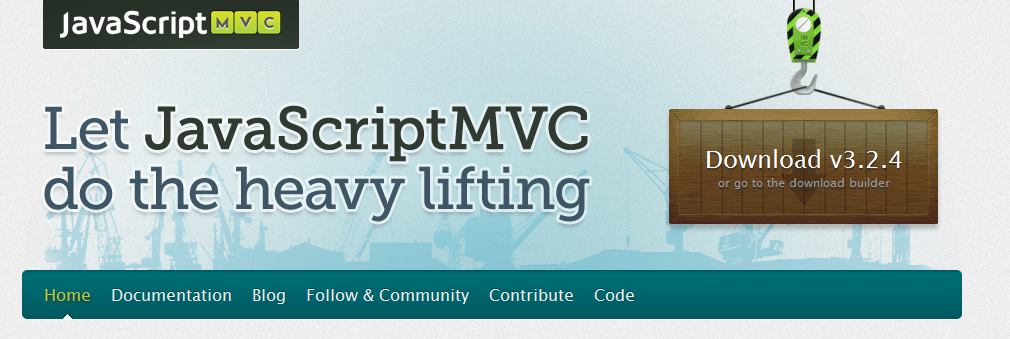
\includegraphics[scale=0.6]{javamvc.png}
			Figure that created by JavaScriptMVC
			\end{center}
		\subsubsection{JQuery}
			\begin{itemize}
				\item Overview: JQuery is free, open source software, licensed under the MIT License. It's also one of the best JavaScript frameworks at presence.
				\item Pros: 
					\begin{itemize}
						\item Easy to use
						\item Large library
						\item Strong community
						\item Great documents and tutorials
						\item Ajax support
					\end{itemize}
				\item Cons:
					\begin{itemize}
						\item Functionality maybe limited
					
					\end{itemize}
			\end{itemize}
			\begin{figure}
				\begin{center}
				\includegraphics[scale=1.2]{jquery.png}
				\caption{An example created by JQuery}
				\end{center}
			
			\end{figure}

		\subsubsection{Cappuccino}
			\begin{itemize}
				\item Overview: an open source framework that makes it easy to build desktop-caliber applications that run in a web browser which look and feel like desktop applications on Mac OS X.
				\item Pros: 
					\begin{itemize}
						\item allow you to create true desktop-like apps right inside the browser
						\item don’t rely on a continous web connection
						\item as fast as desktop app
						\item you can build asyncronous, offline, robust web apps right inside the browser
						\item Cappuccino is compatible with many of the latest browsers
					
					\end{itemize}
				\item Cons:
					\begin{itemize}
						\item Adding a layer of abstraction (Objective-J objects to Javascript) also adds to the overhead. The result is that the application can be slow, particularly if the user's computer is slow.
						\item It is not designed to make full-fledged web sites. That leads to complex and interactive sites may not suitable
						\item is still very early in its development stages, so some parts are still unimplemented
						\item Different Underlying Model
					\end{itemize}
			\end{itemize}
			\begin{figure}
				\begin{center}
				\includegraphics[scale=1.3]{Cappuccino1.png}
				\caption{An example created by cappucino}
				\end{center}
			\end{figure}
		\subsubsection{Ember.js}
			\begin{itemize}
				\item Overview: Ember is a JavaScript framework for creating ambitious web applications that eliminates boilerplate and provides a standard application architecture. Same company with Sproutcore.
				\item Pros: 
					\begin{itemize}
						\item easily implementing MVC functionality.
						\item extremely easy to create computed properties in JavaScript
						\item It is designed so you don't have to worry about whether or not you have 2000 bindings.
						\item is intended for "web-styled" applications.
					\end{itemize}
				\item Cons:
					\begin{itemize}
						\item Documents are not quite clear and understandable.
					
					\end{itemize}
			\end{itemize}
			\begin{figure}
			\begin{center}
			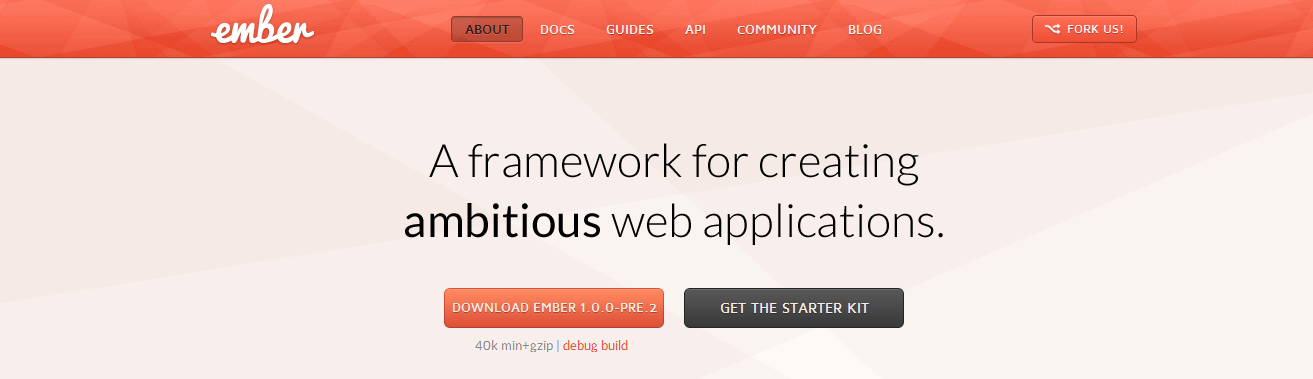
\includegraphics[scale=0.5]{ember.png}
			\caption{An example created by ember}
			\end{center}			
			\end{figure}

		\subsubsection{Flame.js}
			\begin{itemize}
				\item Overview: It's a widget/UI library for Ember.js, so it has all the properties of Ember.js listed above.
				
			\end{itemize}
		\subsubsection{Angular.js}
			\begin{itemize}
				\item Overview:  an open-source JavaScript framework.
				\item Pros: 
					\begin{itemize}
						\item You don't have to write all the event listening and event triggering. Its automatic.
						\item if you want something declarative that uses the View to derive behaviour.
						\item focuses on achieving this through custom HTML tags.
						\item great for small- to intermediate-scale applications
					\end{itemize}
				\item Cons:
					\begin{itemize}
						\item Obtrusively mixes all controller, model and view into the html
						\item invents its own syntax which requires learning
						\item Javascript errors happen if you DON'T clutter the window object.
						\item the more bound elements in your app, the slower it gets
						\item Difficult to allow browsers to optimize this in native code.
						\item It only provides an interface between a combined M, V and C. What if you wanted a Model to subscribe to another Model but didn't want to update a view. You can't do this with Angular.js, but you can with Backbone.
					\end{itemize}
					\begin{figure}
						\begin{center}
							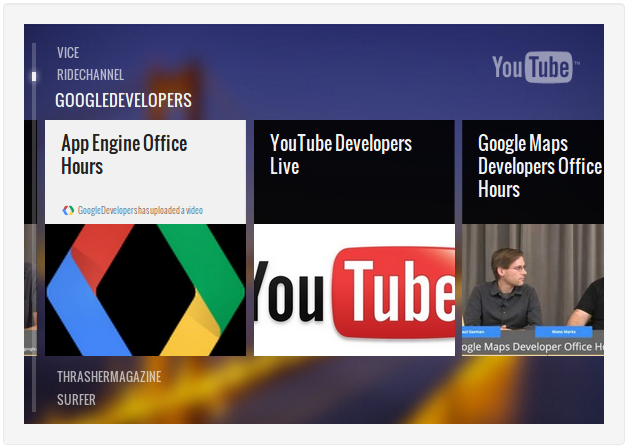
\includegraphics[scale=0.5]{Angular.png}
							\caption{An example created by AngularJS}
						\end{center}
					\end{figure}
			\end{itemize}
		\subsubsection{Twitter Bootstrap}
			\begin{itemize}
				\item Overview:  is a free collection of tools for creating websites and web applications. It contains HTML and CSS-based design templates for typography, forms, buttons, charts, navigation and other interface components, as well as optional JavaScript extensions.
				\item Pros: 
					\begin{itemize}
						\item The framework can be adapted to any CMS or blogging platform like WordPress, Drupal or Joomla.
						\item  Easy visual consistency in your application.
						\item This framework is designed for a web application (not a website) and all the elements fit nicely together to get the app done fast.
						\item many beautiful theme"
						\item Speed, Consistency across applications
						\item People find it simple and elegant"
					\end{itemize}
				\item Cons:
					\begin{itemize}
						\item  incomplete support for HTML5 and CSS 3, but it is compatible with all major browsers.
						\item It uses Less css. but many people like to use other tool to mangage css
					
					\end{itemize}
			\end{itemize}
			\begin{figure}
				\begin{center}
				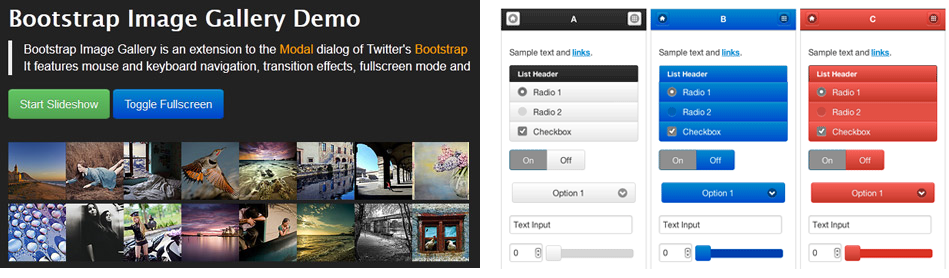
\includegraphics[scale=0.7]{twitter.png}
				\caption{An example that created by Twitter Bootstrap}
				\end{center}				
			\end{figure}

		\subsubsection{Ext JS/Sencha}
			\begin{itemize}
				\item Overview:  a pure JavaScript application framework for building interactive web applications using techniques such as Ajax, DHTML and DOM scripting.
				\item Pros: 
					\begin{itemize}
						\item is like a superset of the widgets like simple label, textbox buttons to complex grids, drag-drop panel
						\item It has quite good documentation with tutorials, samples and user community.
						\item Active and currently most adopted javascript RIA framework
						\item  Good code quality/readability
						\item  Ext JS makes it simple to edit tickets inline
					\end{itemize}
				\item Cons:
					\begin{itemize}
						\item Loading time would is high for home page on web.
						\item CSS – very easy to get lost. It is difficult to find correct class names.
						\item HTML – full of divs and overly complex generated code. Difficult to debug even with FireBug.
						\item  Customization is not easily achievable.
						\item Loading even simple things requires few lines of coding which is simpler in plain html or jQuery
						\item Need quite experienced developer"
					\end{itemize}
			\end{itemize}
			
			\begin{figure}
				\begin{center}
				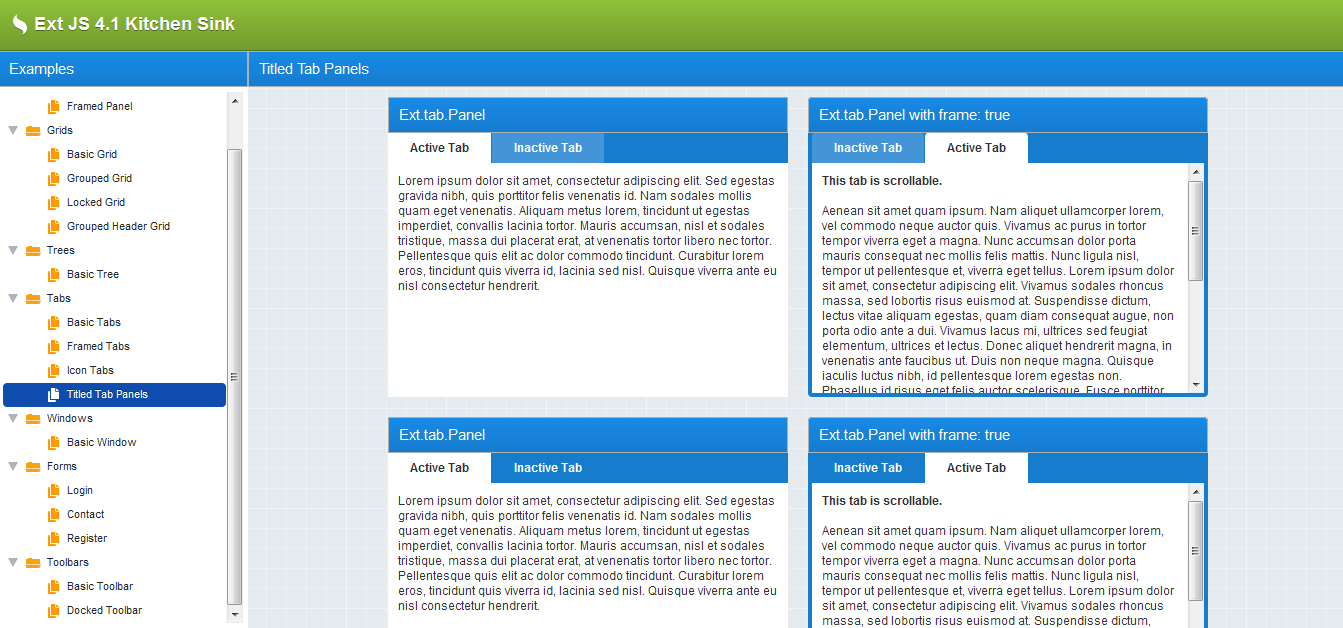
\includegraphics[scale=0.5]{sencha.png}
				\caption{An example that created by sencha}
				\end{center}
			\end{figure}
			
			\begin{figure}
				\begin{center}
				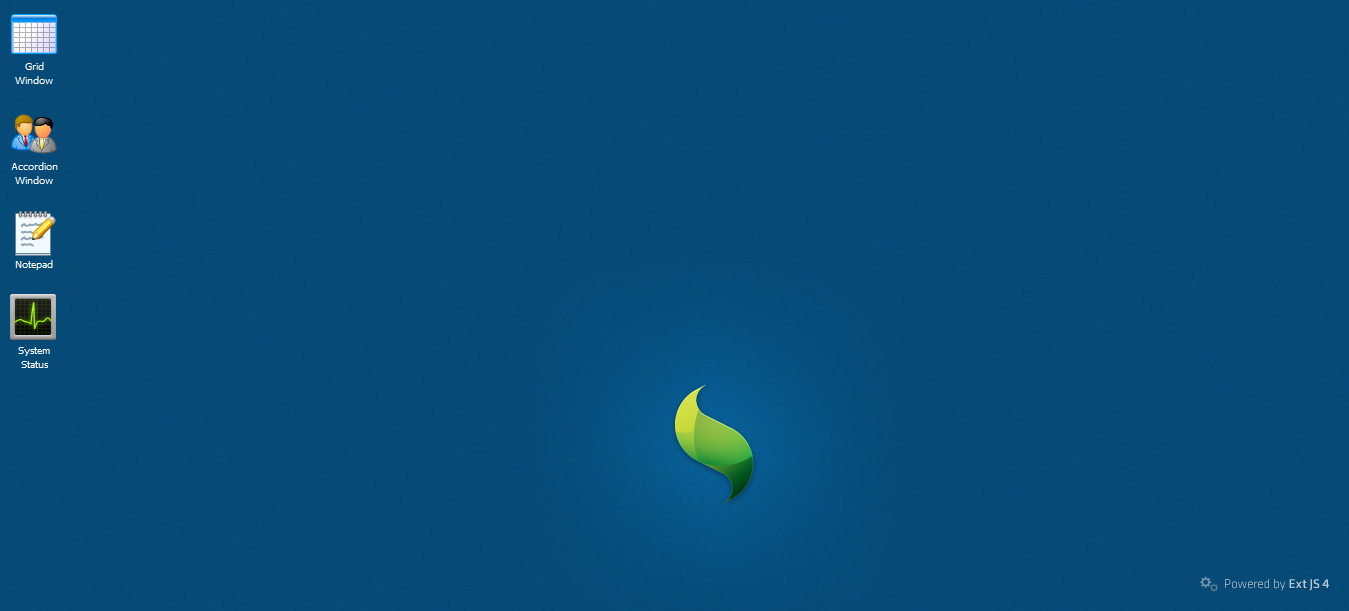
\includegraphics[scale=0.5]{sencha1.png}
				\caption{Another example that created by sencha}
				\end{center}
			\end{figure}					
			
			
		\subsubsection{quooxdoo}
			\begin{itemize}
				\item Overview: ooxdoo is a universal JavaScript framework with a coherent set of individual components and a powerful toolchain
				\item Pros: 
					\begin{itemize}
						\item supports namespace,eventbiding,cross-browser back button, bookmarkability, AOP
						\item feature supports Browser abstraction, DOM manipulation, Events, Templating, Animation.
					\end{itemize}
				\item Cons:
					\begin{itemize}
						\item non CSS -based styling
					
					\end{itemize}
			\end{itemize}
			\begin{figure}
				\begin{center}
				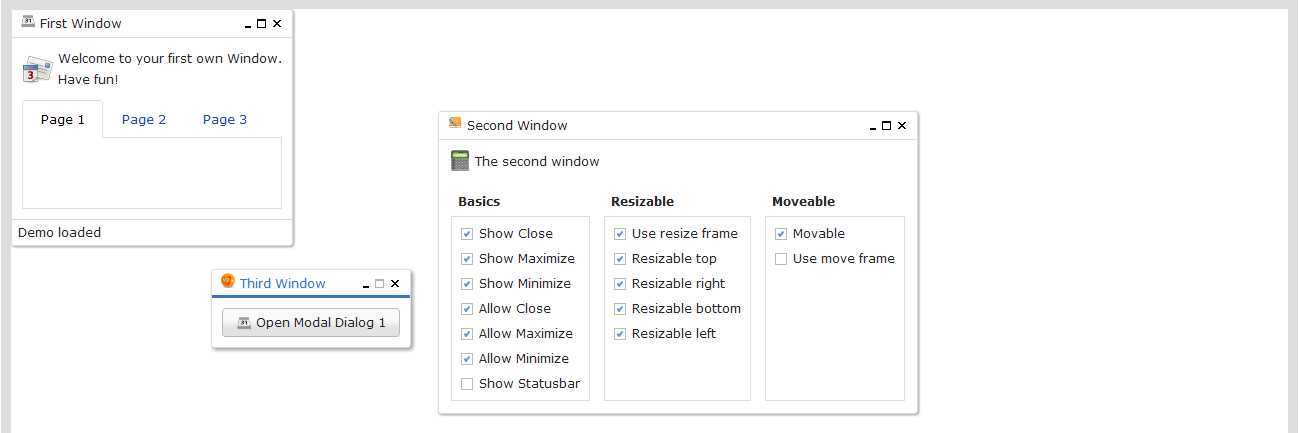
\includegraphics[scale=0.6]{qooxdoo.png}
				\caption{An example that created by qooxdoo}
				\end{center}
			\end{figure}

		\subsubsection{JQueryUI}
			\begin{itemize}
				\item Overview: a curated set of user interface interactions, effects, widgets, and themes built on top of the jQuery JavaScript Library. Whether you're building highly interactive web applications or you just need to add a date picker to a form control, jQuery UI is the perfect choice.
				\item Pros: 
					\begin{itemize}
						\item Base on one of the most popular framework now.
						\item Stable
						\item Nice Theme
						\item support interaction
						\item MIT license
						\item One of the nicest things from jQuery.UI I think is the widget factory, which gives you a quick way of creating your own plug-ins.
						\item is extremely easy to use. Built-in functions are very comprehensive. Compatibility is good.
					\end{itemize}
				\item Cons:
					\begin{itemize}
						\item too heavy
						\item javaScript 's cons
					
					\end{itemize}
			\end{itemize}
			\begin{figure}
				\begin{center}
				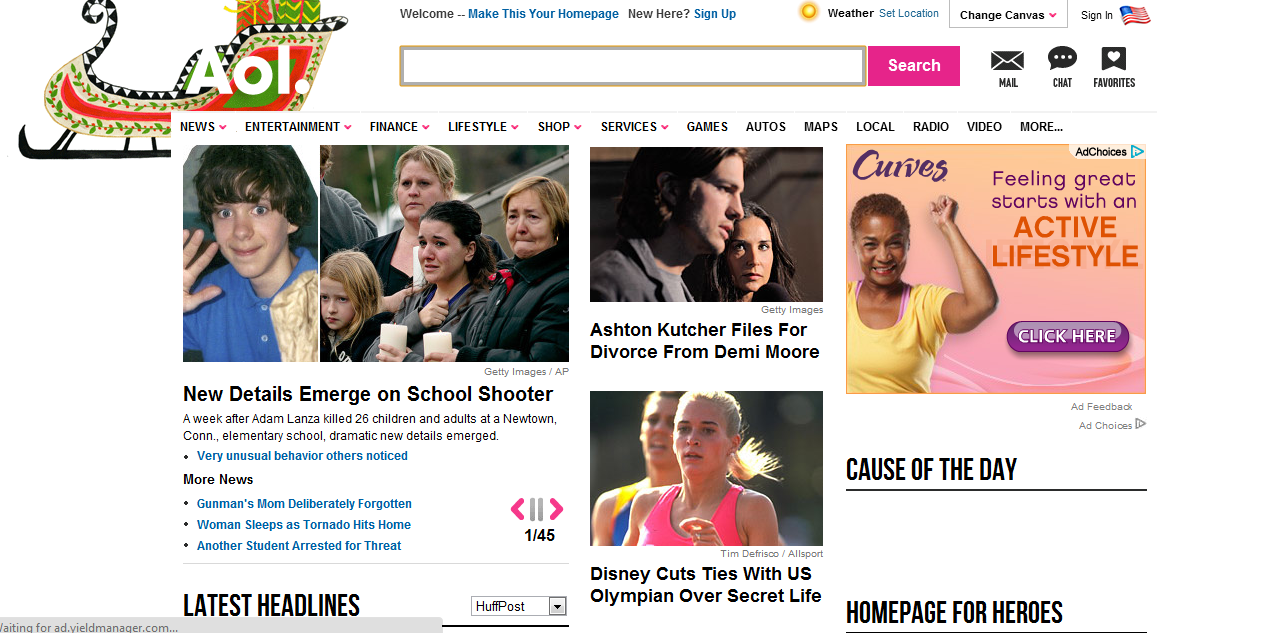
\includegraphics[scale=0.5]{jqueryui.png}
				\caption{An example that created by jqueryui}
				\end{center}
			\end{figure}

		\subsubsection{YUI}
			\begin{itemize}
				\item Overview: an open-source JavaScript library for building richly interactive web applications using techniques such as Ajax, DHTML and DOM scripting.
				\item Pros: 
					\begin{itemize}
						\item support models, views and routers and make it simple to write multi-view applications supporting routing, View transitions and more.
						\item it is a complete solution that includes widgets/components as well as the tools needed to create an organized application architecture.
						\item have scaffolding tools (yuiproject), but these need to be updated
						\item includes all of the goodies of Backbone
					\end{itemize}
				\item Cons:
					\begin{itemize}
						\item it should support some of the auto-wiring (optional) of Ember
						\item should have more AMD-compatible module loader"
					
					\end{itemize}
			\end{itemize}
			\begin{figure}
				\begin{center}
				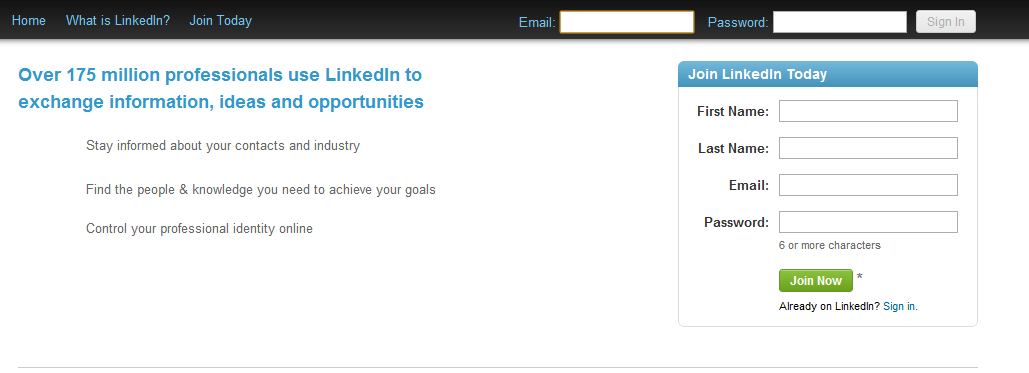
\includegraphics[scale=0.6]{YUI.png}
				\caption{An example that created by YUI}
				\end{center}			
			\end{figure}

			\subsubsection{Backbone.js}
			\begin{itemize}
				\item Overview: Backbone.js gives structure to web applications by providing models with key-value binding and custom events, collections with a rich API of enumerable functions, views with declarative event handling, and connects it all to your existing API over a RESTful JSON interface.
				\item Pros: 
					\begin{itemize}
						\item support a persistence layer and RESTful sync, models, views (with controllers), event-driven communication, templating and routing.
						\item suitable  to build non-trivial applications
						\item quickly depart from one another in how they expect you to approach building apps.
						\item more suitable with something flexible which offers a minimalist solution to separating concerns in my application
						\item you want control, and compatibility with other frameworks.
					\end{itemize}
				\item Cons:
					\begin{itemize}
						\item  A bit clunky, always having to create both the event trigger and event listener in all all view, model, router etc, which makes for larger code and longer figuring it out writing it.
					\end{itemize}
			\end{itemize}
			\begin{figure}
				\begin{center}
				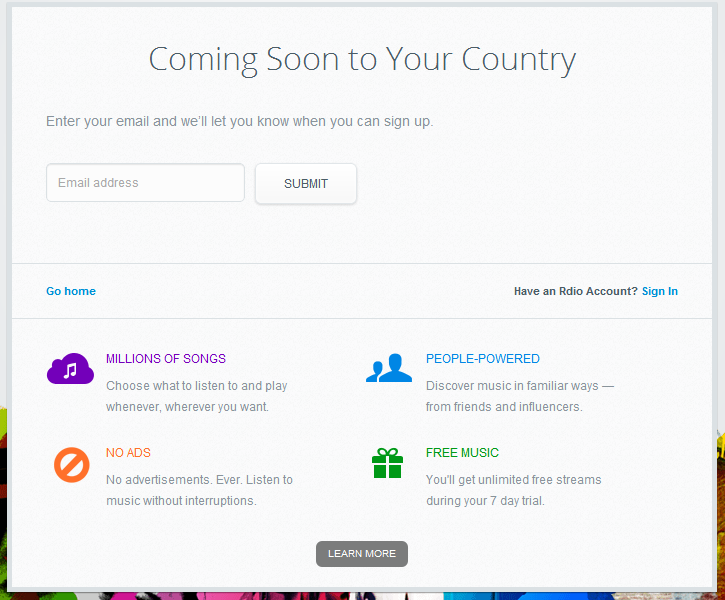
\includegraphics[scale=0.9]{backbone.png}
				\caption{An example that created by backbone}
				\end{center}
			\end{figure}

			\subsubsection{DHTMLX}
			\begin{itemize}
				\item Overview:DHTMLX Touch is an HTML5-based JavaScript library for building mobile web applications. It’s not just a set of UI widgets, but a complete framework that allows you to create eye-catching, cross-platform web applications for mobile and touchscreen devices.
				\item Pros: 
					\begin{itemize}
						\item Great features and UI components.
						\item Great tutorials and samples.
						\item Doesn't conflict with well-known AJAX framework like: JQuery, YUI,..
						\item The library works in all modern browsers: 
						
					\end{itemize}
				\item Cons:
					\begin{itemize}
						\item
					
					\end{itemize}
			\end{itemize}
			\begin{figure}
				\begin{center}
				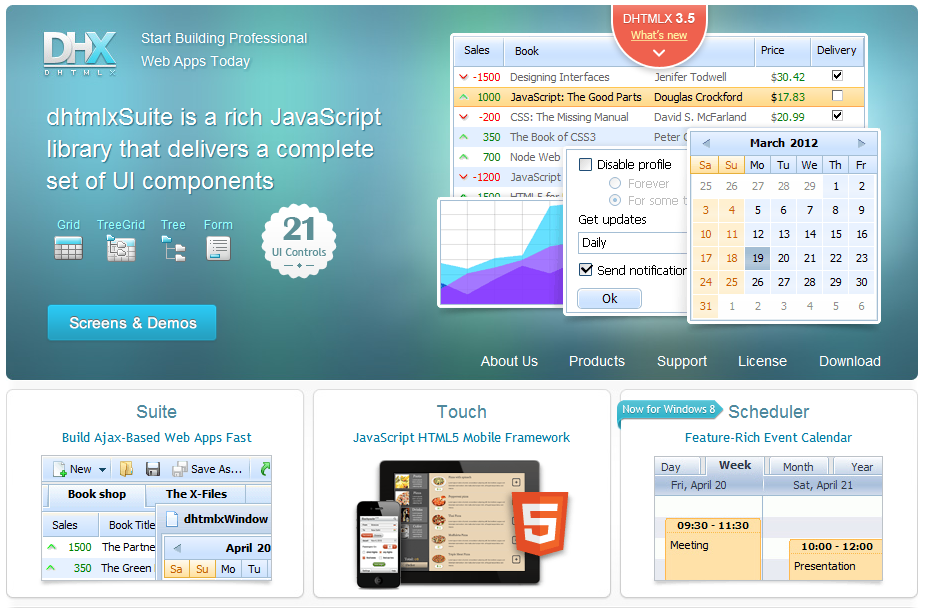
\includegraphics[scale=0.7]{dhtmlx.png}
				\caption{An example that created by DHTMLX}
				\end{center}			
			\end{figure}

			\subsubsection{Rialto}
			\begin{itemize}
				\item Overview: Rialto (Rich Internet Application Toolkit) is a cross browser ajax based JavaScript widgets library. Because it is technology agnostic it can be encapsulated in JSP, JSF, Python, .Net or PHP graphic components.
				\item Pros: 
					\begin{itemize}
						\item is designed for SPA
						\item Widgets library includes: forms, dragdrop, tree, data list with fix header and resizable columns, pop up, splitter.
					\end{itemize}
				\item Cons:
					\begin{itemize}
						\item The documents and demos seem to be vague 
						\item the community is not so active
					
					\end{itemize}
			\end{itemize}
			
The Tables below provide an overview of available MV* frameworks. Columns in the table show the different frameworks, while the  rows classify them with respect to the classification dimensions introduced .The character "x" equals to "yes" and "-" equals to "no". Furthermore additional information for every framework is provided: These following tables show more information about those JavaScript frameworks. The tables also reveal the uniform distribution of MVC and MVVM frameworks as well as JavaScript being the predominant programming language. Furthermore most of the frameworks require no special integration process to be used within an application. Usually it is enough to include a single JavaScript file into the application’s source code. 			
			\begin{table}[ht]
				\begin{center}
					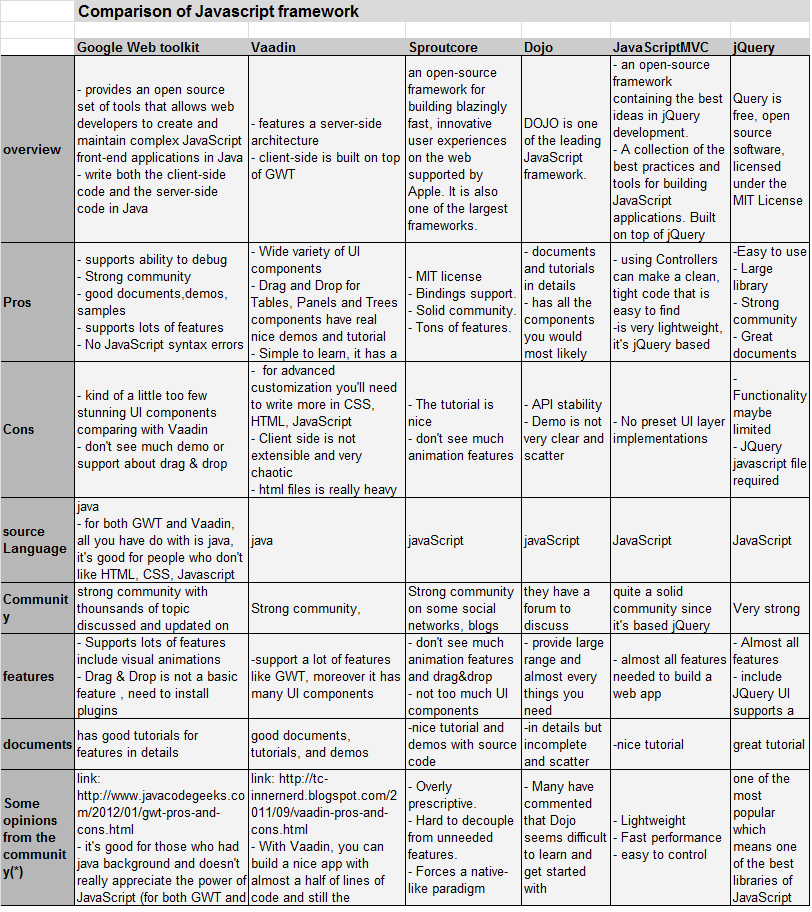
\includegraphics[scale=0.6]{JavaFrameTable1.png}
				
					\caption{Some of JavaScript frameworks in the survey (first six ones)}
				\end{center}
			
			\end{table}
			\begin{table}[ht]
				\begin{center}
					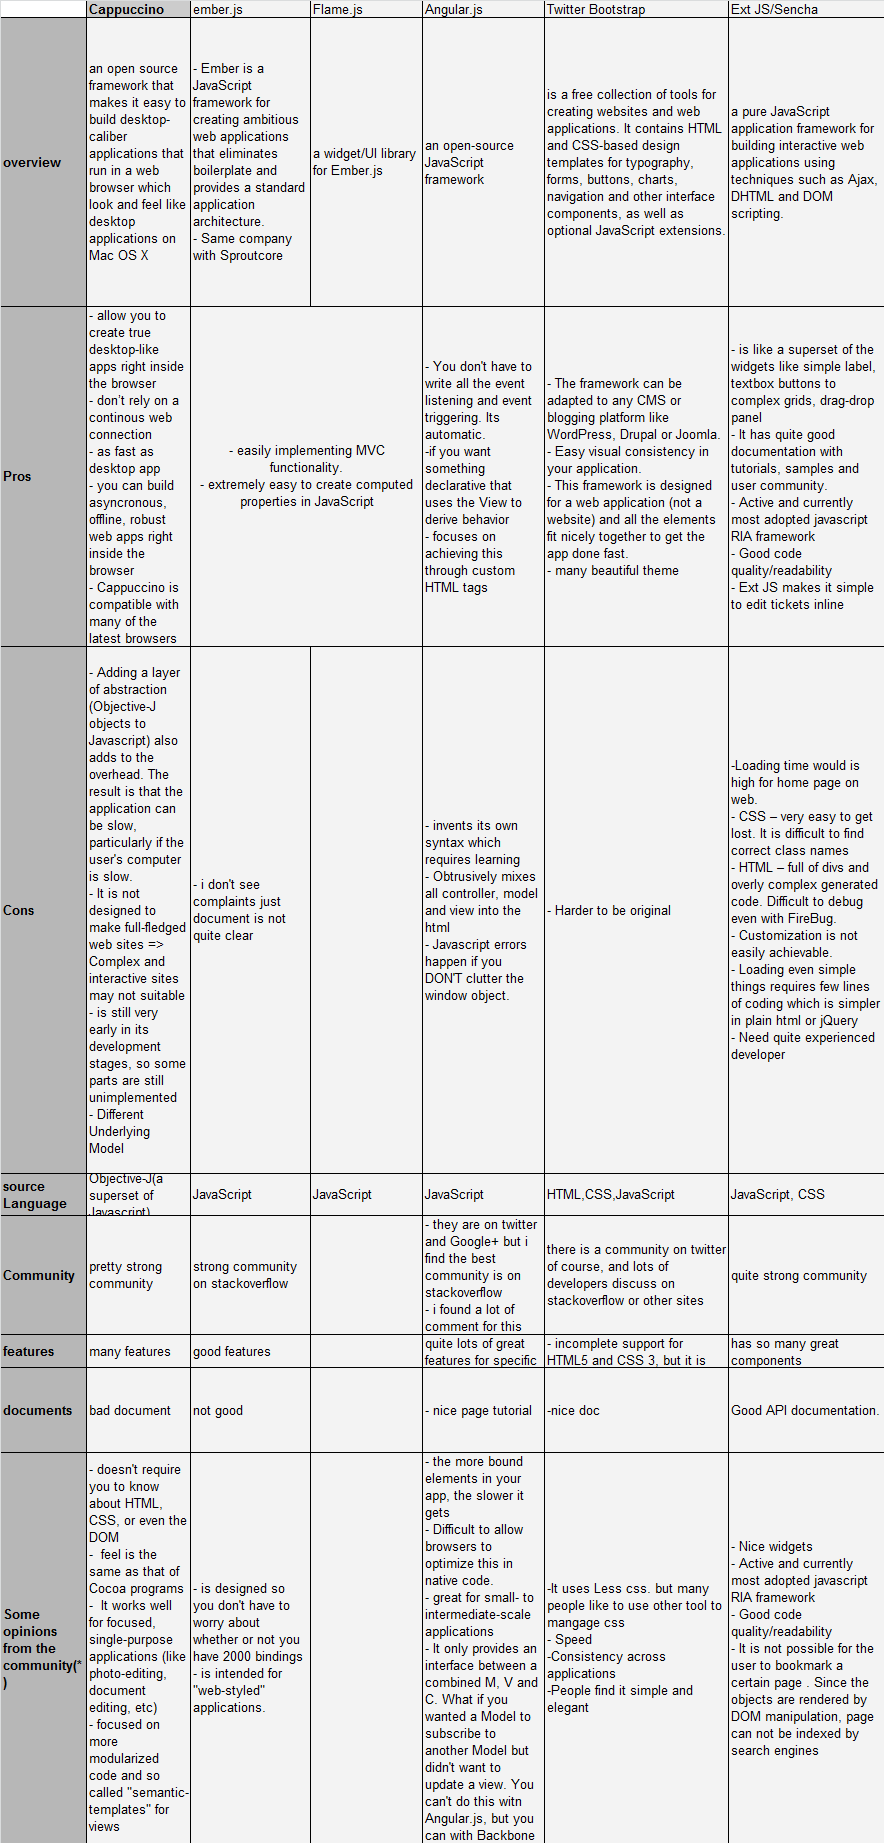
\includegraphics[scale=0.4]{JavaFrameTable2.png}
				
					\caption{Some of JavaScript frameworks in the survey (second six ones)}
				\end{center}
			
			\end{table}
			
			\begin{table}[ht]
				\begin{center}
					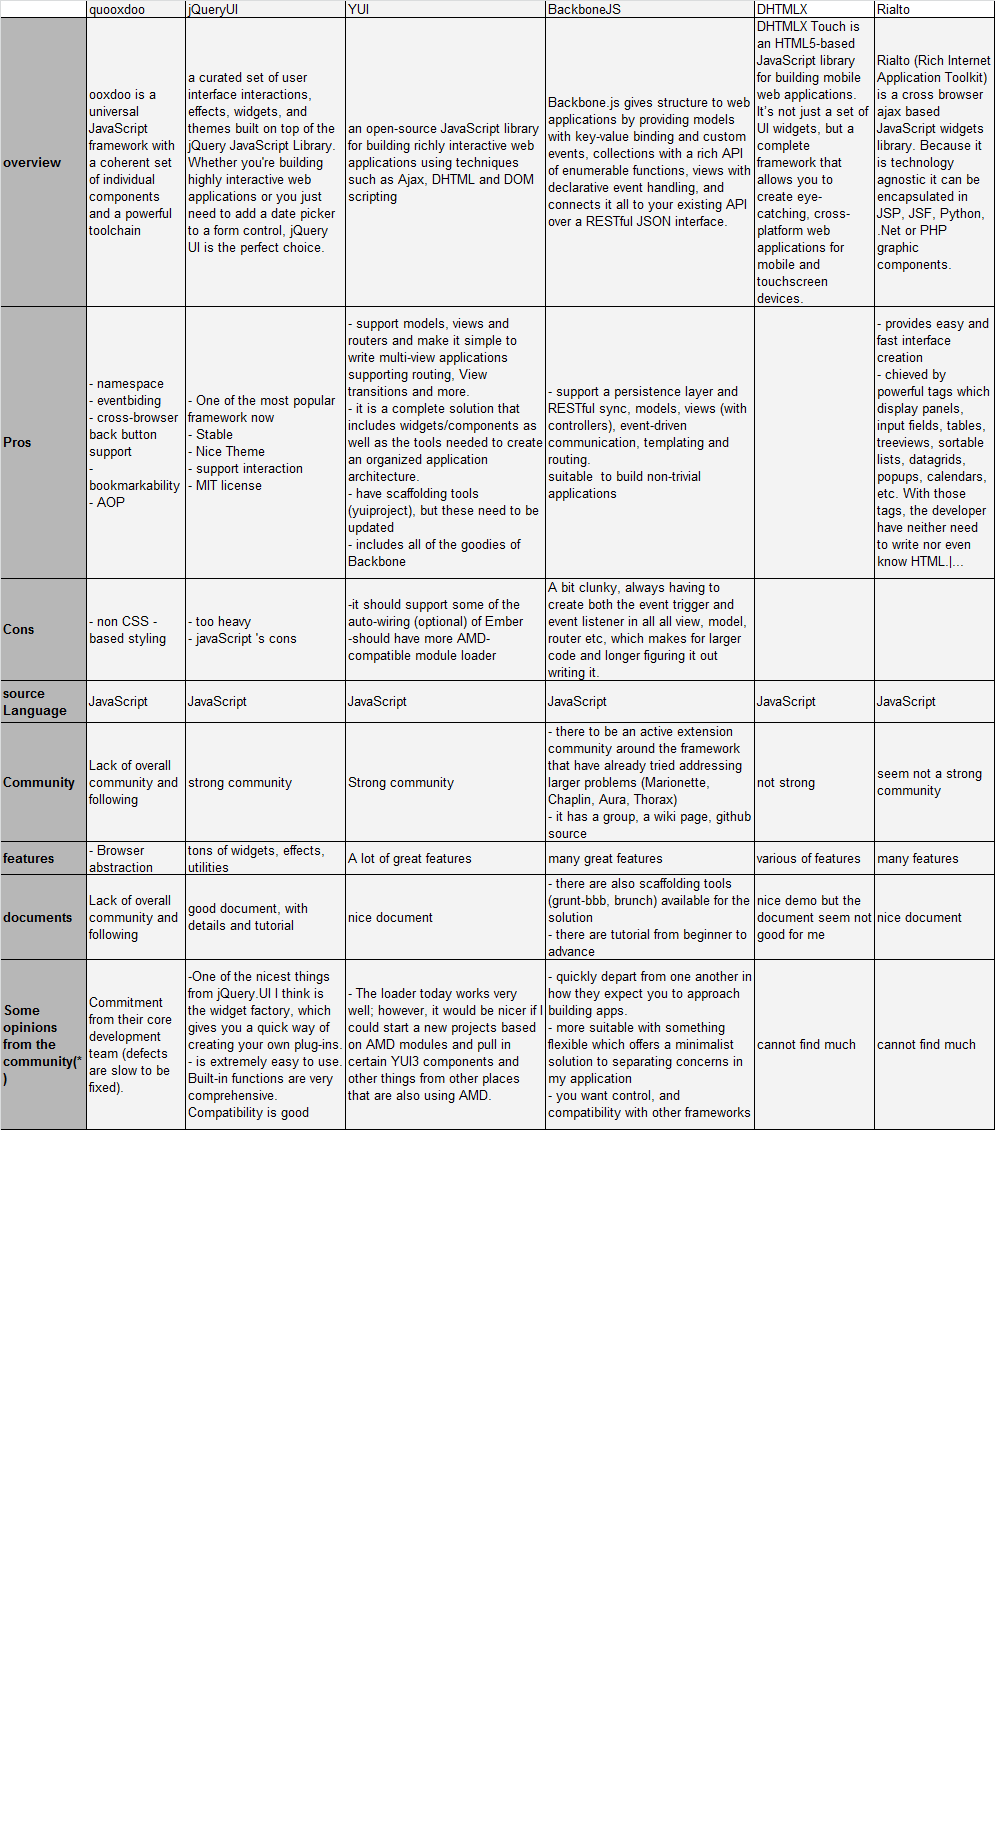
\includegraphics[scale=0.4]{JavaFrameTable3.png}
				\caption{Some of JavaScript frameworks in the survey(third six ones)}
				\end{center}
			
			\end{table}
			
			\begin{table}[ht]
				\begin{center}
					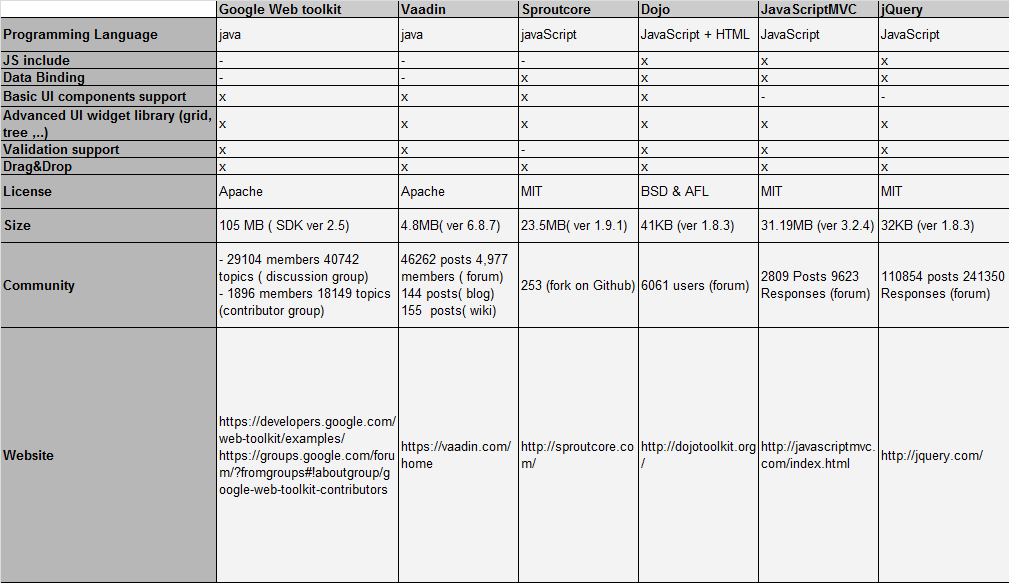
\includegraphics[scale=0.6]{JavaFrameTable1NewCriteria.png}
				
					\caption{First six JavaScript frameworks surveyed with new criteria}
				\end{center}
			
			\end{table}
			\begin{table}[ht]
				\begin{center}
					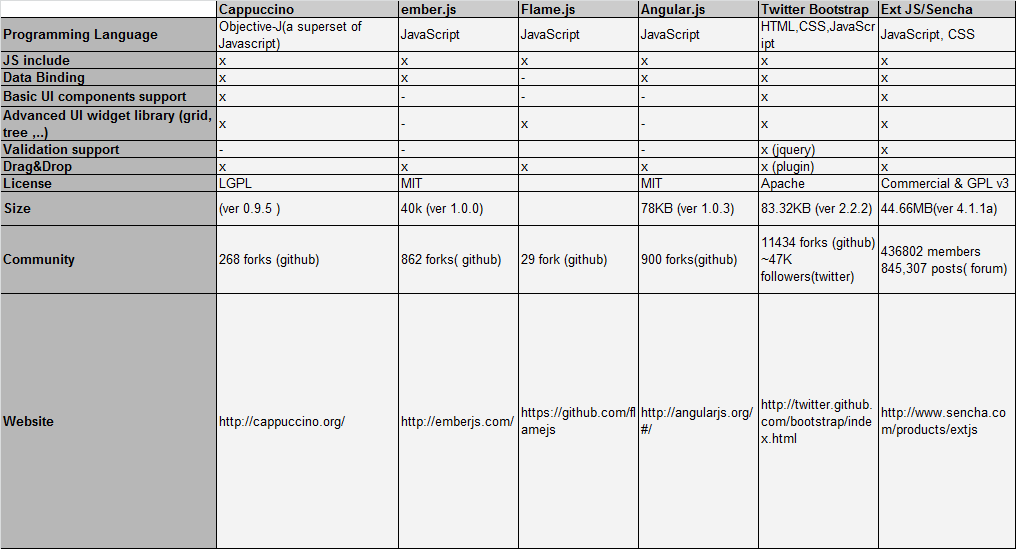
\includegraphics[scale=0.6]{JavaFrameTable2NewCriteria.png}
				
					\caption{Second six JavaScript frameworks surveyed with new criteria}
				\end{center}
			
			\end{table}
			\begin{table}[ht]
				\begin{center}
					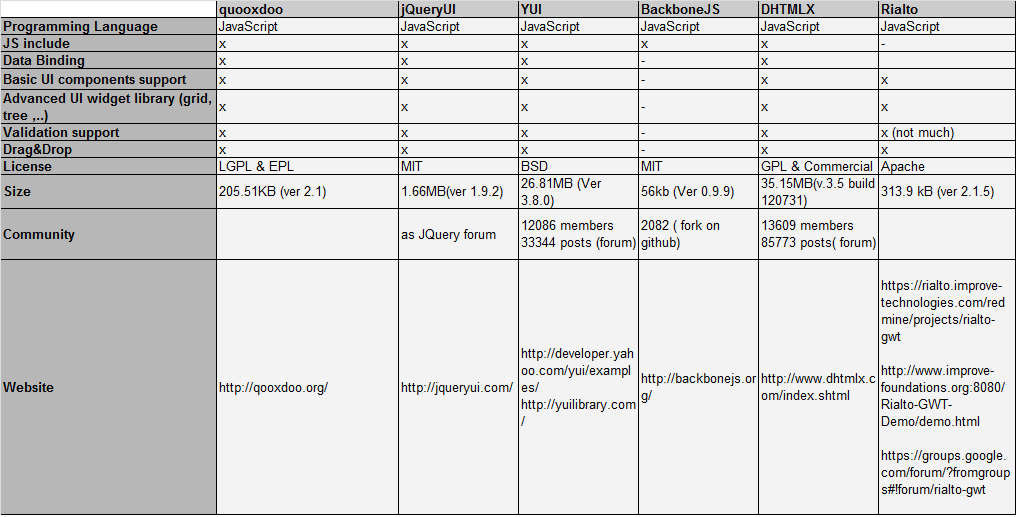
\includegraphics[scale=0.6]{JavaFrameTable3NewCriteria.png}
				
					\caption{First six JavaScript frameworks surveyed with new criteria}
				\end{center}
			
			\end{table}


		\subsection{Selected Framework}
			\subsubsection{Angular.js}
		Angular.js is a JavaScript framework released under the open source MIT license. The implementation is based on JavaScript and has a very small footprint (78 kB minified). Since Angular.js has no dependencies it can be used in conjunction with any other JavaScript library. For developers a very comprehensive set of documentation is available comprising an API specification, interactive tutorials as well as running examples. Moreover, Angular.js is special JavaScript framework which is built particularly for software engineering purpose.Angular.js lets you extend HTML vocabulary for your application. The resulting environment is extraordinarily expressive, readable, and quick to develop.Besides, Angular.js is designed from ground up to be testable. It encourages behavior-view separation, comes pre-bundled with mocks, and takes full advantage of dependency injection. It also comes with end-to-end scenario runner which eliminates test flakiness by understanding the inner workings of AngularJS.
					
 	\section{JavaScript Graph Libraries Selection}
 		\subsection{Overview of some javaScript Graph libraries}
 		There are several graph libraries providing APIs for implementing and managing various kinds of diagram. Among them , there are some names that have been used a lot like Joinjs, mxgraph,Yfiles, Draw2D. While some of them have just been introduced like Gojs, Raphael, d3js. They are all remarkable libraries which provide stunning UI and animations. It would be hard to choose one of them if there are not criteria a to compare. Therefore, the some criteria will be presented in the next section.
 			
	 			 			
		\subsection{JavaScript Graph Libraries Selection Characteristics} 		
		These are some criteria that will be based on to choose graph library
		\begin{itemize}
		\item Language: javaScript
		\item Feature supports various types of shapes
		\item Drag \& drop support
		\item data binding support
		\item Light weight and easy to integrate
		\item Nice designed documents and lots of samples
		\item The license under which the framework is released
		\item The size of the library
		\item Community: the number of users or posts in the forum they use or on GitHub( Jan 2013) indicating the community support, as well as the website of the framework usually providing tutorials and a more or less comprehensive documentation.
		\end{itemize}
		\subsection{Survey of Existing graph libraries }
		Conducting a survey about JavaScript graph libraries is an inevitable step before choosing one library for implementation. This survey provides an overview of what these libraries are capable of and base on that a library will be chosen with the features fit the most with the proposed criteria.
 			
			\subsubsection{JoinJS}
 				JointJS is an open source modern JavaScript library for creating diagrams. It can be used to create either static diagrams or, and more importantly, fully interactive diagramming tools and application builders.
 				\begin{figure}[ht]
 					\begin{center}
 						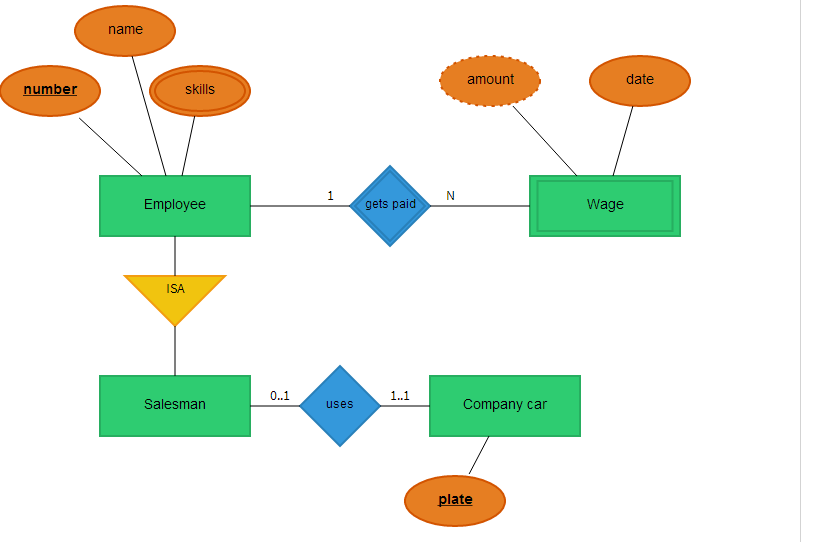
\includegraphics[scale=0.5]{joinjs.png}
 						\caption{A sample created by JoinJS}
 					\end{center}
 				\end{figure}
 			\subsubsection{mxGraph}
 			mxGraph is an interactive JavaScript HTML 5 diagramming library, with full fallback support for IE 6-8. mxGraph is simple, you include it as a JavaScript link in your HTML file and you instantly have access to the cleanest, most functional native browser diagramming component available. Draw.io\footnote{https://www.draw.io/} is a great demo built by Google inc using mxGraph library.
 				\begin{figure}[ht]
 					\begin{center}
 						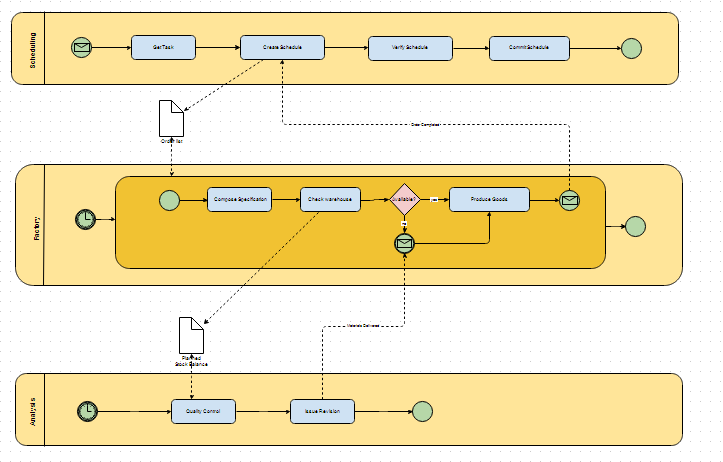
\includegraphics[scale=0.5]{mxgraph.png}
 						\caption{A sample created by mxgraph}
 					\end{center}
 				\end{figure}
 			\subsubsection{YFiles}
 			yFiles for HTML brings the proven power and ease of yFiles diagramming to your cutting-edge HTML5 applications. yFiles for HTML has almost all functionality known from our diagramming libraries for the .NET platform. It contains UI controls for viewing and editing diagrams and our layout algorithms for automatically arranging complex graphs and networks at the click of a button.
				\begin{figure}[ht]
 					\begin{center}
 						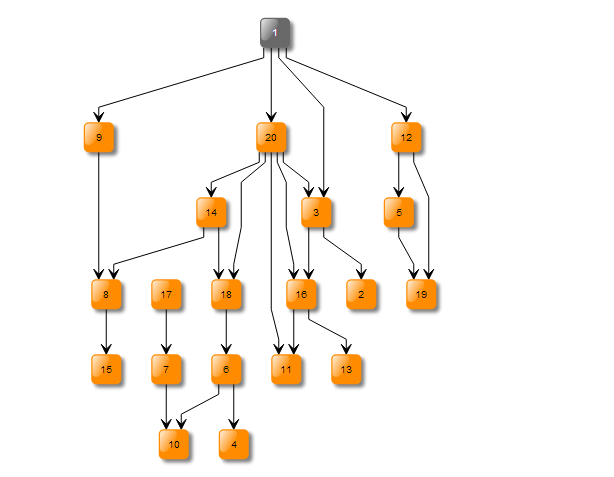
\includegraphics[scale=0.5]{yfiles.png}
 						\caption{A sample created by yFiles}
 					\end{center}
 				\end{figure} 			
 			\subsubsection{Canviz}
 			Canviz is a JavaScript library for drawing Graphviz graphs to a web browser canvas. More technically, Canviz is a JavaScript xdot renderer. It works in most modern browsers.
				\begin{figure}[ht]
 					\begin{center}
 						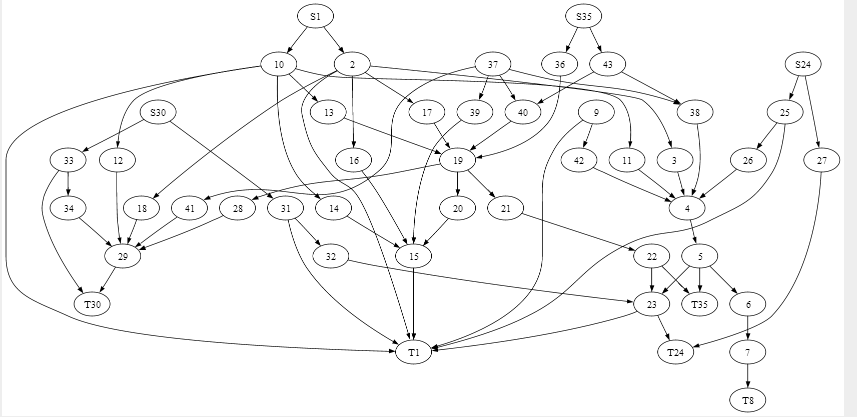
\includegraphics[scale=0.5]{canviz.png}
 						\caption{A sample created by canviz}
 					\end{center}
 				\end{figure} 			
 			
 			\subsubsection{Draw2D}
 			Create drawings, diagrams or an workflow editor with the Javascript library. The User interface allows interactive drawing by using your standard browser.
 			\begin{figure}[ht]
 					\begin{center}
 						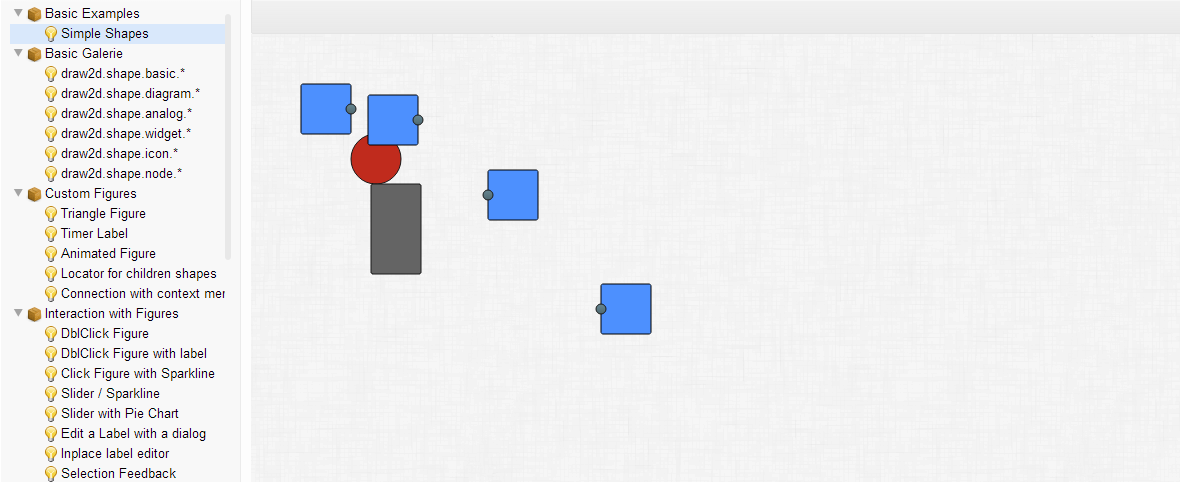
\includegraphics[scale=0.5]{draw2d.png}
 						\caption{A sample created by draw2D}
 					\end{center}
 				\end{figure} 	
 			\subsubsection{Data-driven documents}
 			D3.js is a JavaScript library for manipulating documents based on data. D3 helps you bring data to life using HTML, SVG and CSS. D3’s emphasis on web standards gives you the full capabilities of modern browsers without tying yourself to a proprietary framework, combining powerful visualization components and a data-driven approach to DOM manipulation.
 			  	\begin{figure}[ht]
 					\begin{center}
 						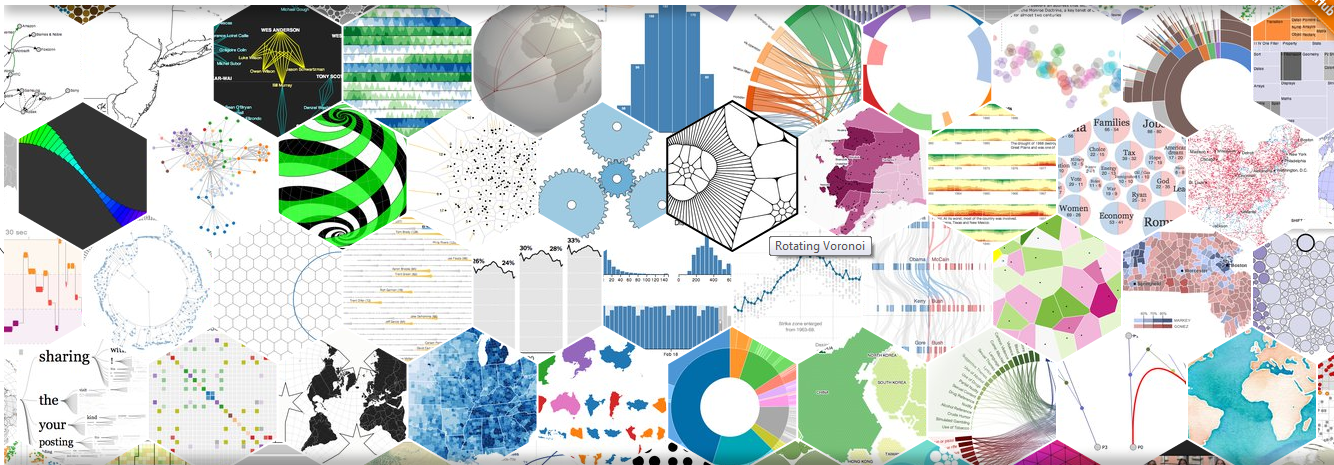
\includegraphics[scale=0.5]{d3js.png}
 						\caption{A sample created by D3js}
 					\end{center}
 				\end{figure} 	
 			
 			\subsubsection{Gojs}
 			GoJS is a feature-rich JavaScript library for implementing interactive diagrams across modern browsers and platforms. GoJS makes constructing diagrams of complex Nodes, Links, and Groups easy with customizable templates and layouts.
 			\begin{figure}[ht]
 					\begin{center}
 						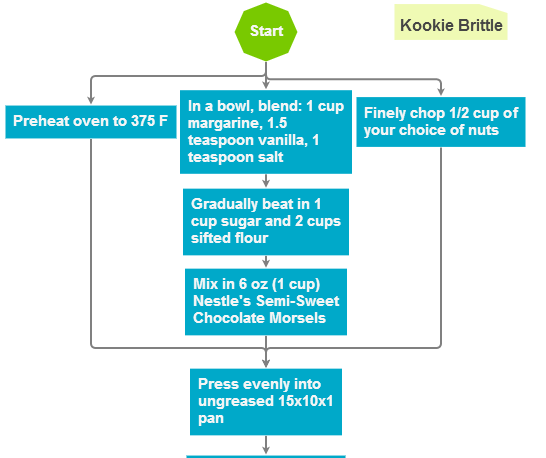
\includegraphics[scale=0.5]{gojs.png}
 						\caption{A sample created by Gojs}
 					\end{center}
 				\end{figure} 	
 			\subsubsection{mindfusion}
 			The library is written 100\% in JavaScript and uses the HTML5 Canvas element for drawing. JsDiagram depends on the Microsoft Ajax® library for type system implementation and browser independence. With JSDiagram users can create, resize, select, move and modify nodes and links as they wish. You can allow or permit any action or customize how the control response to a certain action - like pressing the 'Del' key for example.
 			\begin{figure}[ht]
 					\begin{center}
 						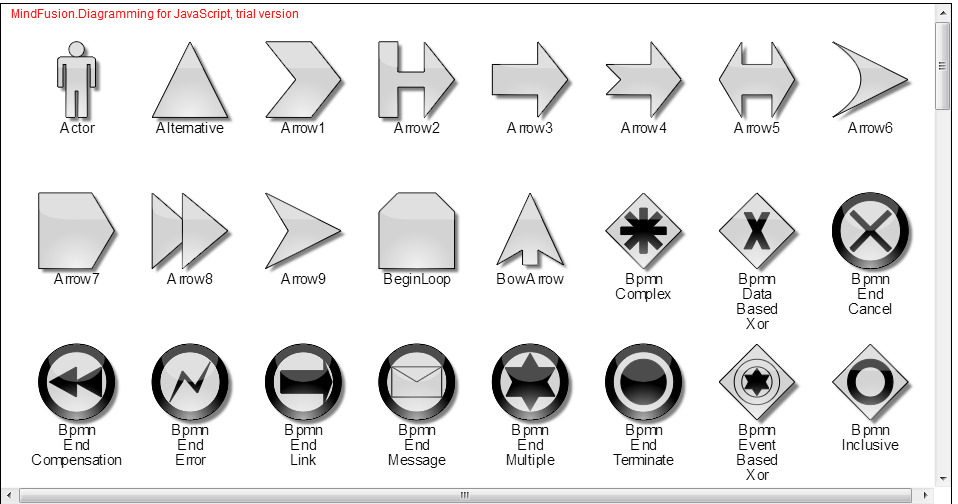
\includegraphics[scale=0.5]{mindfusion.png}
 						\caption{A sample created by Mindfusion}
 					\end{center}
 				\end{figure} 
 			
 			\subsubsection{Raphael}
 			Raphaël is a small JavaScript library that should simplify your work with vector graphics on the web. If you want to create your own specific chart or image crop and rotate widget, for example, you can achieve it simply and easily with this library.
 			\begin{figure}[ht]
 					\begin{center}
 						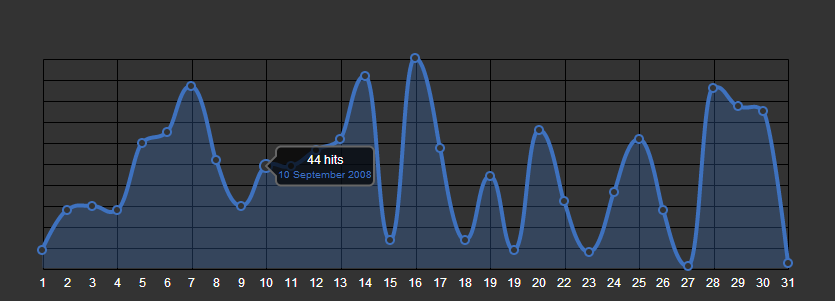
\includegraphics[scale=0.5]{rafael.png}
 						\caption{A sample created by Raphael}
 					\end{center}
 				\end{figure} 
 			
 			\subsubsection{JavaScript InfoVis Toolkit}
				The JavaScript InfoVis Toolkit provides tools for creating Interactive Data Visualizations for the Web.
				\begin{figure}[ht]
 					\begin{center}
 						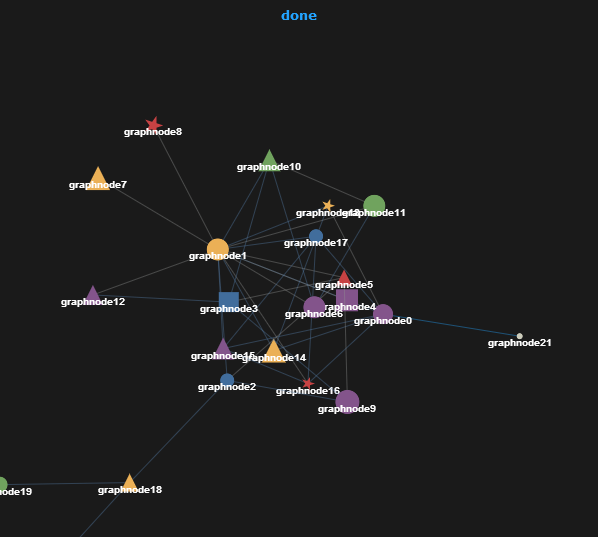
\includegraphics[scale=0.5]{JIT.png}
 						\caption{A sample created by JavaScript InfoVis Toolkit}
 					\end{center}
 				\end{figure} 
				
 			\subsubsection{jsUML2}
 			jsUMLT2 is a lightweight HTML5/javascript library for UML 2 diagramming. It allows the developer to easily embed UML 2 diagram in web applications, just invoking a few javascript methods.
 			\begin{figure}[ht]
 					\begin{center}
 						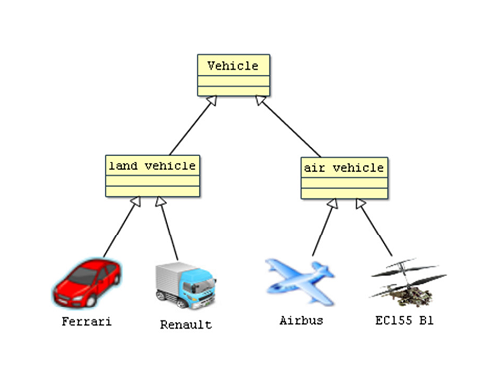
\includegraphics[scale=0.5]{jsUML2.png}
 						\caption{A sample created by jsUML2}
 					\end{center}
 				\end{figure} 
 			\subsubsection{JsPlumb}
 			jsPlumb allows you to connect elements on the screen using SVG, Canvas or VML, depending on the capabilities of the browser. go with jQuery/MooTools/YUI3.
 			\begin{figure}[ht]
 					\begin{center}
 						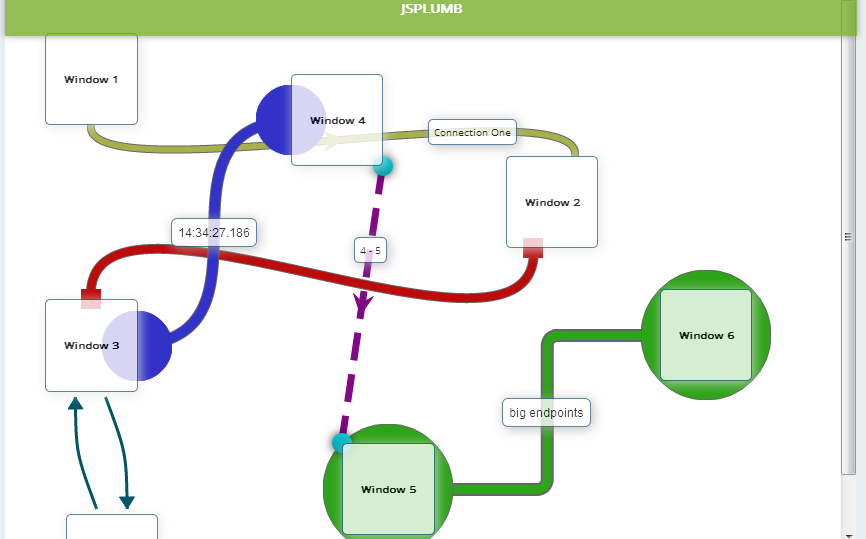
\includegraphics[scale=0.5]{jsplumb.png}
 						\caption{A sample created by jsPlumb}
 					\end{center}
 				\end{figure} 
 			\subsubsection{Nodeviz}
 			NodeViz includes PHP code for managing assembling relational data on a server, formatting it for Graphviz network layout, sending SVG or JPG versions of the network to client, JavaScript classes for embedding network graph image and associated lists in client web page, as well as methods and events for zooming, panning, highlighting and other interactions.
 			
 			The two following table ~\ref{graphfirst7} and table ~\ref{graphrest} show the information of all JavaScript graph libraries which were surveyed.
 			
 			\begin{table}[ht]
 				\begin{center}
 					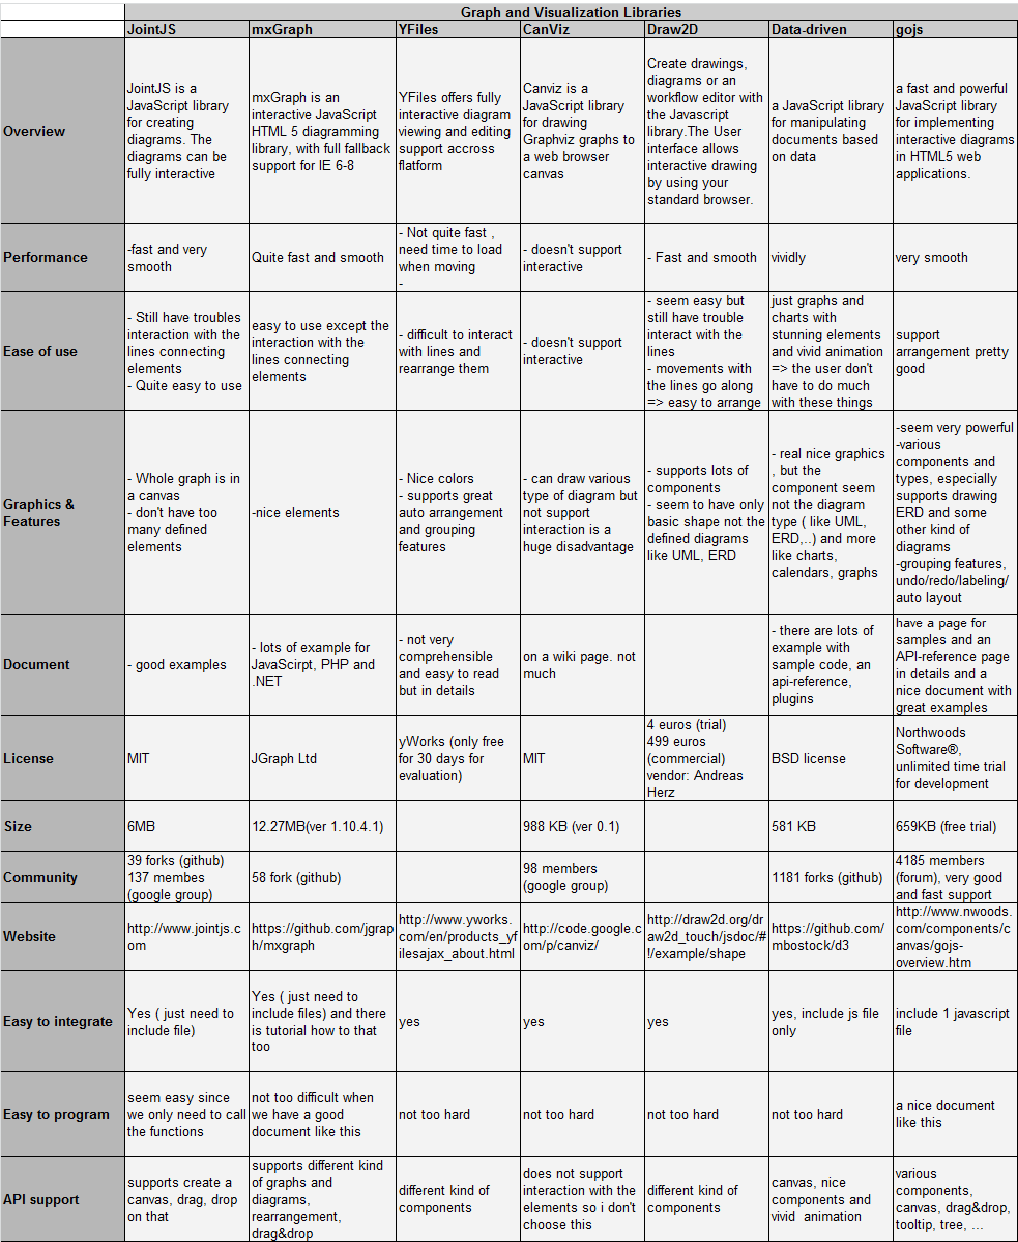
\includegraphics[scale=0.5]{GraphLibrary1.png}
 					\caption{Survey information of first sevens javascript graph libraries }
 					\label{graphfirst7}
 				\end{center}
 			\end{table}
 			
 			 \begin{table}[ht]
 				\begin{center}
 					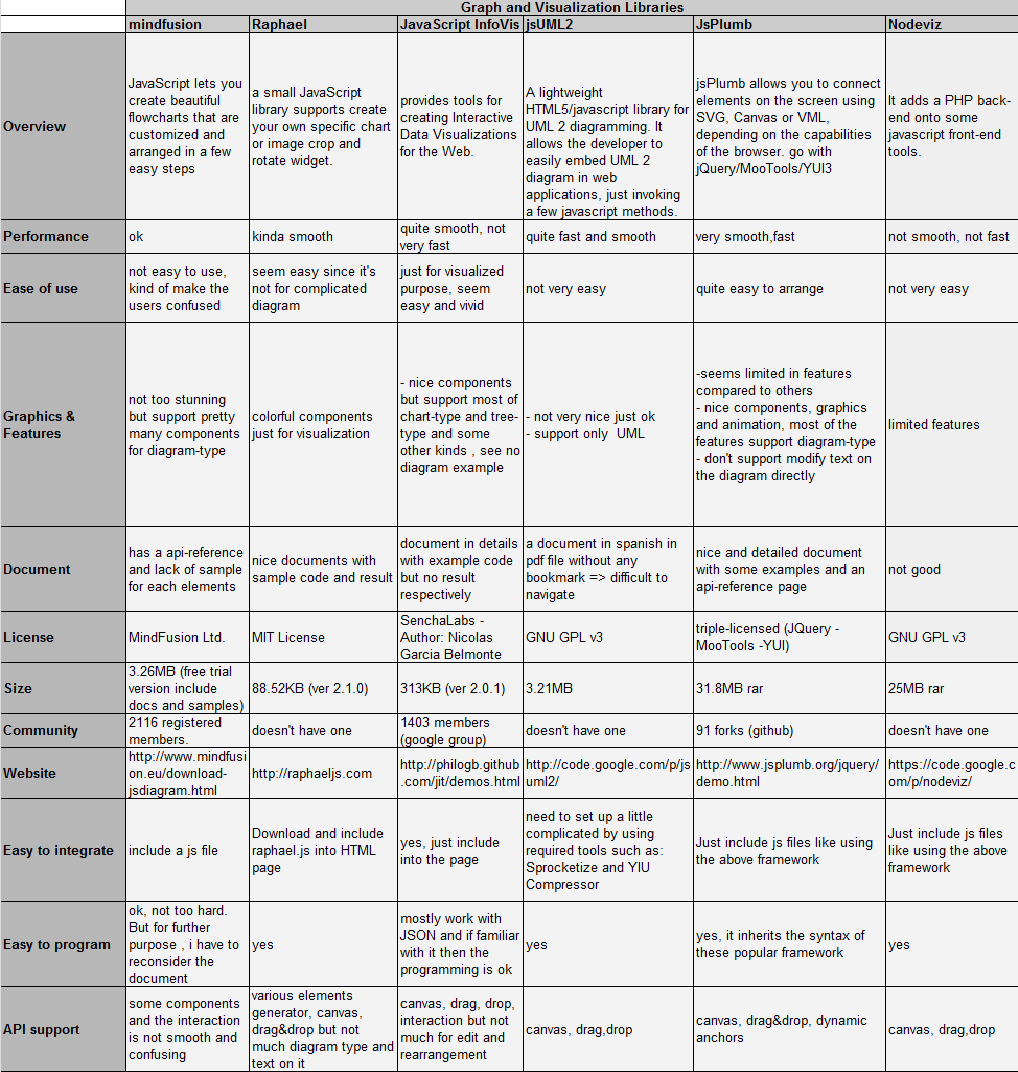
\includegraphics[scale=0.5]{GraphLibrary2.png}
 					\caption{Survey information of the rest of graph libraries }
 					\label{graphrest}
 				\end{center}
 			\end{table}
		\subsection{Selected graph library}	
			\subsubsection{Gojs}
			Gojs is a fast and powerful JavaScript library for implementing interactive diagrams in HTML5 web applications. it is released under nwoods company license. The reason Gojs is chosen it that this library is a new product and providing such beautiful graphics and various kind of sample shapes. The implementation is based on JavaScript and has a small footprint (659KB (free trial)). Since Gojs has no dependencies it can be integrated with Angular.js. For developers there is an in-details introduction, a lot of sample code and demos. Besides, there is a forum for developers to ask question and it is well-replied by the admins of the site. 
				

\chapter{EXPLORATION OF KEY TECHNOLOGIES}
\textsl{In this chapter, I will present all the key technologies that i have been using in this thesis. For each technology, a brief overview will be introduced as well as their main features, advantages. Some important concept are also presented}
\newpage

	\section{AngularJS}
		\subsection{overview}
		AngularJS is a structural framework for dynamic web apps. It lets you use HTML as your template language and lets you extend HTML's syntax to express your application's components clearly and succinctly. Out of the box, it eliminates much of the code you currently write through data binding and dependency injection. And it all happens in JavaScript within the browser, making it an ideal partner with any server technology.
\\		

Angular is what HTML would have been had it been designed for applications. HTML is a great declarative language for static documents. It does not contain much in the way of creating applications, and as a result building web applications is an exercise in what do I have to do to trick the browser into doing what I want.
\\

The impedance mismatch between dynamic applications and static documents is often solved with:
\begin{itemize}
\item a library - a collection of functions which are useful when writing web apps. Your code is in charge and it calls into the library when it sees fit. E.g., jQuery.
\item frameworks - a particular implementation of a web application, where your code fills in the details. The framework is in charge and it calls into your code when it needs something app specific. E.g., knockout, ember, etc.

\end{itemize}


Angular takes another approach. It attempts to minimize the impedance mismatch between document centric HTML and what an application needs by creating new HTML constructs. Angular teaches the browser new syntax through a construct we call directives. Examples include:

\begin{itemize}
\item Data binding, as in \{\{\}\}.
\item DOM control structures for repeating/hiding DOM fragments.
\item Support for forms and form validation.
\item Attaching code-behind to DOM elements.
\item Grouping of HTML into reusable components.

\end{itemize}
		
		\subsection{Why Angular?}
			\subsubsection{DECLARATIVE HTML APPROACH}
			Declarative programming is when you say what you want, and imperative language is when you say how to get what you want. 

Let’s take an example:
			\begin{verbatim}
			# Declarative
small_nums = [x for x in range(20) if x < 5]

# Imperative
small_nums = []
for i in range(20):
 if i < 5:
 small_nums.append(i)
			\end{verbatim}
			\subsubsection{ANGULARJS $‘$S PHILOSOPHY}
The AngularJS philosophy is based on embracing and extending HTML, while meeting the needs of both new and experienced developers. Moreover, Angular is built around the belief that declarative code is better than imperative when it comes to building UIs and wiring software components together, while imperative code is excellent for expressing business logic.
			
		\subsection{Dependency Injection}
			\subsubsection{Introduction}
			There are only three ways an object or a function can get a hold of its dependencies:
\begin{enumerate}
\item The dependency can be created, typically using the new operator or asking a factory object to make one.
\begin{verbatim}
public SomeClass() {

 myObject = new Object(objectname);

}

public SomeClass() {

 myObject = Factory.getObject(objectname);

}
\end{verbatim}
\item The dependency can be looked up by referring to a global variable.
\begin{verbatim}
public SomeClass() {

 myObject = GLOBAL_OBJECT;

}
\end{verbatim}
\item The dependency can be passed in to where it is needed.
\begin{verbatim}
public SomeClass (Object myObject) {

 this.myObject = myObject;

}
\end{verbatim}

\end{enumerate}

The first two option are quite bad. Hardcoding the \emph{objectname} does not really solve the problem as you cannot easily change your mind later without changing the that class again. Using a constant \emph{GLOBAL\_OBJECT} is also a bad idea as the \emph{SomeClass} now depends on a constant to be set.
\\

But there is yet another problem that cannot be solved easily: How can I change Object class? For instance, to replace it with a mock object to ease testing. This makes the class difficult to modify the dependencies. This is especially problematic in tests, again ,where it is often desirable to provide mock dependencies for test isolation[].
\\

The third option , which simply passed the dependencies into where it is needed , is the most viable, since it removes the responsibility of locating the dependency from the component. The dependency is simply handed to the component.That's Dependency Injection. Nothing more! Using the SomeClass class is now a bit more 
involving as you first need to create the object:
\begin{verbatim}
myObject = new Object(objectname);

someInstance = new SomeClass(myObject);
\end{verbatim}
Basically, DI can be simply explained as follow, instead of having the objects creating a dependency or asking a factory object to make one for them, you pass the needed dependencies in to the constructor, and you make it somebody else's problems . One of the major advantages of dependency injection is that it can make testing lots easier. 
\\

This is just for your first sight of what will happen to the code and how it looks like when we use DI. I’ll explain why we are doing this and its benefits later. First, let’s see what is the definition of this design pattern.

			\subsubsection{Definition}
			Dependency injection (DI) is a software design pattern that allows removing hard-coded dependencies and making it possible to change them, whether at run-time or compile-time[1]

Dependency injection involves at least three elements:
\begin{itemize}
\item a dependent consumer,
\item a declaration of a component's dependencies, defined as interface contracts,
\item an injector (sometimes referred to as a provider or container) that creates instances of classes that implement a given dependency interface on request.
\end{itemize}

The dependent object describes what component it depends on to do its work. The injector decides what concrete classes satisfy the requirements of the dependent object, and provides them to the dependent.
\\

Being able to make this decision at run-time rather than compile time is the key advantage of dependency injection. Multiple, different implementations of a single software component can be created at run-time and passed (injected) into the same test code. The test code can then test each different software component without 
being aware that what has been injected is implemented differently.
			\subsubsection{Types}
			Dependency Injection is not restricted to constructor injection:

\begin{itemize}
\item Constructor injection
\begin{verbatim}
public SomeClass {

	SomeClass(myObject){
	
		 this.myObject = myObject;
		 
	}
}
\end{verbatim}
\item Setter Injection:
\begin{verbatim}
public SomeClass {

	public Setter(myObject){
	
		 this.myObject = myObject;
		 
	}
}
\end{verbatim}
\item  Property Injection:
\begin{verbatim}
public SomeClass {

	public ObjectProperty;
	
}

someClass->ObjectProperty = property;
\end{verbatim}
\end{itemize}
		\subsubsection{Benefits}
\begin{itemize}
\item Reduction of boilerplate code – which is included in many places without any alteration and the programmers have to write more code to do minimum jobs in the application objects since all work to initialize or set up dependencies is handled by a provider component . 
\item Very useful when we have objects whose implementations change often 
\item Very useful for large projects where there is issue of maintainability, simplicity.

\item Useful in unit testing, as it is easy to inject a fake implementation of a service into the object being tested by changing the configuration file, or overriding component registrations at run-time.

\item Dependency Injection facilitates the writing of testable code.
\end{itemize}
			\subsubsection{Examples and explanation in AngularJS}
			\begin{verbatim}
1.	function SomeClass(greeter) {
2.	this.greeter = greeter;
3.	}
4.	 
5.	SomeClass.prototype.doSomething = function(name) {
6.	this.greeter.greet(name);
7.	}
\end{verbatim}
In the above example SomeClass is not concerned with locating the greeter dependency, it is simply handed the greeter at runtime.This is desirable, but it puts the responsibility of getting hold of the dependency on the code that constructs SomeClass.To manage the responsibility of dependency creation, each Angular application has an injector. The injector is a service locator that is responsible for construction and lookup of dependencies.
\begin{verbatim}
1.	// Provide the wiring information in a module
2.	angular.module('myModule', []).
3.	 // Teach the injector how to build a 'greeter'
4.	// Notice that greeter itself is dependent on '$window'
5.	factory('greeter', function($window) {
6.	// This is a factory function, and is responsible for 
7.	// creating the 'greet' service.
8.	return {
9.	greet: function(text) {
10.	$window.alert(text);
11.	}
12.	};
13.	});
14.	 // New injector is created from the module. 
15.	// (This is usually done automatically by angular bootstrap)
16.	var injector = angular.injector(['myModule', 'ng']);
17.	 // Request any dependency from the injector
18.	var greeter = injector.get('greeter');

\end{verbatim}

		\subsection{Separation of Concern}
			\subsubsection{Introduction - What is Separation of Concerns?}
			Development today is not what it used to be. Applications are often far too large for any one person to maintain. Most large applications now require fairly large development teams just to keep them running. The applications they develop get bigger and bigger, application structure and organization grow in importance.Therefore, we need a way to organise and separate components of the application which will make the code maintainable, easily accessible and better performanced.
\\			

There is a typical example that you can have a look for your first image what separation of concerns is. Have you ever see a site where HTML, CSS, JavaScript are all mixed together in one single file and all the components are glued like a mess. And it’s a nightmare to make change or develop any part of that site.
	\subsubsection{A Bad Example where the separation of concerns is violated}
	\begin{verbatim}
		<a href="/some/url/"onclick="someFunction(); return false;" style="font-size: 12px; color: #f00;">A bad link</a>
	\end{verbatim}
	\subsubsection{Good Example}
	In this good example the same thing is done with a clear separation between content, style and behavior.
	\begin{list}{•}{•}
		\item HTML
		\begin{verbatim}
			<a href="/some/url/" id="some_link">A good link</a>
		\end{verbatim}
		\item CSS
		\begin{verbatim}
			#some_link { font-size: 12px; color: #f00; }
		\end{verbatim}				
		\item JavaScript
		\begin{verbatim}
document.getElementById('some_link').addEventListener('click', someFunction, false);		
		\end{verbatim}
	\end{list}
			\subsubsection{Definition}
Separation of Concerns (SoC)  is a standard practice of dividing up major components of an application and segregating them from the rest of the application. There are many different ways to accomplish SoC and one of them is to utilize the magic of Dependency Injection (DI). SoC via DI is the practice of splitting up the application into components, and then resolving any dependencies those components have on other components through the use of injection. For now, you don’t need to worry about what DI is, i’ll explain this concept in another place.

			\subsubsection{Benefits}
		\begin{itemize}
		\item Allow people to work on individual pieces of the system in isolation.
		\item To enable everyone to better understand the system.
		\item To facilitate reusability simplifying development and maintenance of computer programs. When concerns are well separated, individual sections can be developed and updated independently.
		\item the ability to later improve or modify one section of code without having to know the details of other sections, and without having to make corresponding changes to those sections.
		\end{itemize}
			\subsubsection{Example of Separation of Concerns in AngularJs}
			This is an unit test example within the Test Driven Development(TDD) process, in which we will write the unit tests before writing anything else. This can only achieved by implementing Separation of Concerns
			\\
			We can declare what we want in our view:
			\begin{verbatim}
			<a href="/hello" when-active>Hello</a>
			\end{verbatim}
			
			Okay, now we can write a test:
			\begin{verbatim}
			it( 'should add "active" when the route changes', inject(function() {
  var elm = $compile( '<a href="/hello" when-active>Hello</a>' )( $scope );

  $location.path('/not-matching');
  expect( elm.hasClass('active') ).toBeFalsey();

  $location.path( '/hello' );
  expect( elm.hasClass('active') ).toBeTruthy();
}));

			\end{verbatim}
			We run our test and confirm that it fails. So now we can write our directive:
			\begin{verbatim}
			.directive( 'whenActive', function ( $location ) {
  return {
    scope: true,
    link: function ( scope, element, attrs ) {
      scope.$on( '$routeChangeSuccess', function () {
        if ( $location.path() == element.attr( 'href' ) ) {
          element.addClass( 'active' );
        } else {
          element.removeClass( 'active' );
        }
      });
    }
  };
});

			\end{verbatim}
		\subsection{Inversion of Control}
			\subsubsection{Introduction}
			Inversion of control (IoC) is not a new term in computer sciences anymore, although it’s still a pretty new topic in software development. This term was first brought by Martin Fowler in 1988[4] and it’s sometime referred as the Hollywood Principle [4] which states “Don't call us, we'll call you". I found this more obscure and hard to understanding if i throw a definition in the first stage when someone just tries to get what is it. Therefore, there will an example and explanation before we ‘re going to the definition of IoC.
\\			

Let’s see this example, say my app has a diagram editor and to implement this diagram editor i use the gojs library ‘s APIs. In this case, i hard code the class of object that i use to this App class and handle everything. This is what the could look likes when we work in the procedure process.

		\begin{verbatim}
		public class App
{
    private GojSDiagram Diagram;
    public App()
    {
        Diagram = new GojSDiagram ();
    }
}
		\end{verbatim}
		In an IoC scenario we would instead do something like this:
		\begin{verbatim}
			public class App
{
    private GojSDiagram Diagram;
    public App(GojSDiagram  Diagram)
    {
        this.Diagram = Diagram;
    }
}
		\end{verbatim}
		Now, the client creating the App class has the control over which Diagram implementation to use. We're injecting the App with the dependency. If you ‘ve read about the Dependency injection (DI) , you may say that this example of IoC is kind similar to DI. And the answer is yes it is, in fact DI is a special kind of IoC and it’ s a way to implement IoC.
			\subsubsection{Definition}
“Inversion of Control is an abstract principal describing an aspect of some software architecture design in which the flow of control of a system is inverted in comparison to procedural programming.”[6]
			\subsubsection{Benefits}
		This is the main reason why we have to understand these obscure definition and take our time to read about IoC. These are the advantages what IoC can bring to your applicaiton
			\begin{itemize}
			\item Flexibility - Changing the implementation class for a widely used interface is simpler (e.g. replace a mock web service by the production instance)
			\item Readability - the project has one unified and consistent component model and is not littered with factories. The code is briefer and is not littered without dependency lookup code 
			\item Testability - dependencies are easy to replace mocks when they're exposed through a constructor or setter. Easier testing leads to more testing. More testing leads to better code quality, lower coupling, higher cohesion
			\end{itemize}
	
		\subsection{Angular 's key features}
			\subsubsection{Directives}
				One of the best parts of Angular is that you can write your templates as HTML. You can
do this because at the core of the framework we’ve included a powerful DOM transformation engine that lets you extend HTML’s syntax.
\\
Angular comes with many directives that help you define the view for your app. We’ll see more of them soon. These directives can define what we commonly view as the template. They can declaratively set up how your application works or be used to create reusable components.
\\

And you’re not limited to the directives that Angular comes with. You can write your
own to extend HTML’s template abilities to do anything you can dream of.	
\\

A basic pseudo-code template for creating any directive follows: 
\begin{verbatim}
var myModule = angular.module(...);
myModule.directive('namespaceDirectiveName', function factory(injectables) {
 var directiveDefinitionObject = {
   restrict: string,
   priority: number,
   template: string,
   templateUrl: string,
   replace: bool,
   transclude: bool,
   scope: bool or object,
   controller: function controllerConstructor($scope,
                                              $element,
                                              $attrs,
                                              $transclude),
   require: string,
   link: function postLink(scope, iElement, iAttrs) { ... },
   compile: function compile(tElement, tAttrs, transclude) {
     return {
       pre: function preLink(scope, iElement, iAttrs, controller) { ... },
       post: function postLink(scope, iElement, iAttrs, controller) { ... }
     }
   }
 };
 return directiveDefinitionObject;
});
\end{verbatim}			
The following table provides an overview of when you would use each of the options.
\begin{table}[ht]
	\begin{center}
		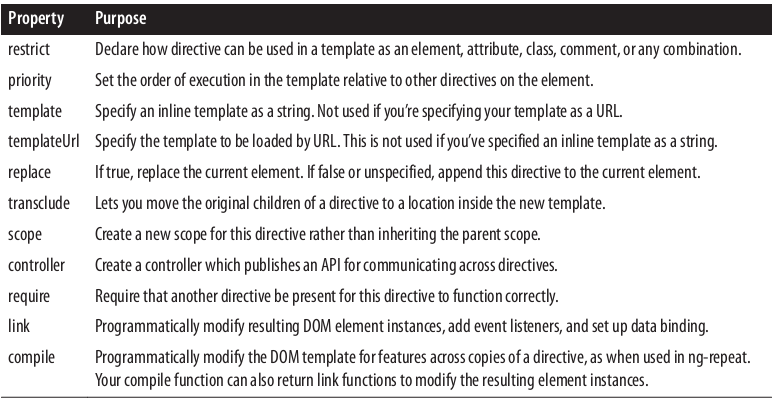
\includegraphics[scale=0.7]{DirectiveDefOpt.png}
		\caption{Directive definition options}
	\end{center}
\end{table}
			\subsubsection{Two-way DataBinding}
				Data-binding in Angular web apps is the automatic synchronization of data between the 
model and view components. The way that Angular implements data-binding lets you treat the model as the single-source-of-truth in your application. The view is a projection of the model at all times. When the model changes, the view reflects the change, and vice versa.
			\begin{itemize}
			\item One-way databinding
			Most templating systems bind data in only one direction (as in ~\ref{fig:onewaydatabinding}): they merge template and model components together into a view, as illustrated in the diagram. After the merge occurs, changes to the model or related sections of the view are NOT automatically reflected in the view. Worse, any changes that the user makes to the view are not reflected in the model. This means that the developer has to write code that constantly syncs the view with the model and the model with the view.
			\begin{figure}
				\begin{center}
					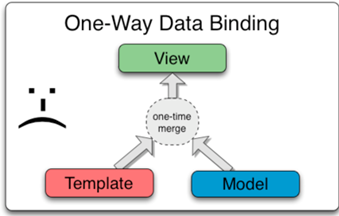
\includegraphics[scale=1]{onewaydatabinding.png}
					\caption{one-way databinding}
					\label{fig:onewaydatabinding}
				\end{center}
			\end{figure}
			\item Two-way databinding
			The way Angular templates works is different, as illustrated in ~\ref{fig:twowaydatabinding}. They are different because first the template (which is the uncompiled HTML along with any additional markup or directives) is compiled on the browser, and second, the compilation step produces a live view. We say live because any changes to the view are immediately reflected in the model, and any changes in the model are propagated to the view.
			\begin{figure}
				\begin{center}
					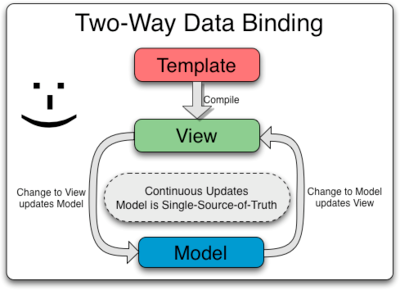
\includegraphics[scale=1]{twowaybinding.png}
					\caption{two-way databinding}
					\label{fig:twowaydatabinding}
				\end{center}
			\end{figure}
			\end{itemize}
			\subsubsection{MVC}
			MVC application structure was introduced in the 1970s as part of Smalltalk[]. From its start in Smalltalk, MVC became popular in nearly every desktop development environment where user interfaces were involved. Whether you were using C++, Java, or Objective-C, there was some flavor of MVC available. Until recently, however, MVC was all but foreign to web development.
\\

The core idea behind MVC is that you have clear separation in your code between managing its data (model), the application logic (controller), and presenting the data to the user (view). Code for AngularJS applications is always organized into models, views, controllers, and (optionally) services.
\\

Models are JavaScript objects that represent the data your application can access. Models are also used to represent the application's current state.
\\

Views play two important roles. First, they are responsible for presenting the data from your models to the user in a visual and useful format. Second, they intercept generic user interactions–including clicks and option list selections–and translate them into application-specific actions. Views in AngularJS are defined declaratively using HTML and CSS.
\\

Controllers define the actual behavior of your application (also called "application logic") and play a key role in connecting the right models to the right views.
\\

Services are specialized objects that perform work on behalf of other objects. Services have many uses, from fetching remote data to providing an implementation of a useful algorithm. Services are intended to be highly reusable and are designed to be swapped easily with other similar services. This concept will be presented more in details in the next part.

			\subsubsection{Services}
			Services are a feature that Angular brings to client-side web apps from the server side, where services have been commonly used for a long time. Services in Angular apps are substitutable objects that are wired together using dependency injection (DI).
\\
			
While Angular offers several useful services, for any nontrivial application you'll find it useful to write your own custom services. To do this you begin by registering a service factory function with a module either via the Module\#factory api or directly via the \$provide api inside of module config function.
\\
c
Example of Using the angular.Module api:
\begin{verbatim}
1.	var myModule = angular.module('myModule', []);
2.	myModule.factory('serviceId', function() {
3.	  var shinyNewServiceInstance;
4.	  //factory function body that constructs shinyNewServiceInstance
5.	  return shinyNewServiceInstance;
6.	});
\end{verbatim}
Using the \$provide service:
\begin{verbatim}
1.	angular.module('myModule', [], function($provide) {
2.	  $provide.factory('serviceId', function() {
3.	    var shinyNewServiceInstance;
4.	    //factory function body that constructs shinyNewServiceInstance
5.	    return shinyNewServiceInstance;
6.	  });
7.	});
\end{verbatim}


			\subsubsection{Unit Testing}
			With the rapid development of software industry, more and more huge applications are produced. Going along with that is a problem how to know the quality of the software products or services before publishing them? That is where software testing taking places. In fact testing is an investigation including several processes whose purpose is to provide an objective, independent view of the software to allow the business to appreciate and understand the risks of software implementation[].
\\

Unit testing, also known as component testing, refers to tests that verify the functionality of a specific section of code, usually at the function level. In an object-oriented environment, this is usually at the class level, and the minimal unit tests include the constructors and destructors[2].  Unit testing is usually performed by the developers working on the code themselves to verify the functions meet their design and behave as intended. There may be multiple tests on one function in order to catch all the cases. Unit testing alone cannot verify the functionality of a piece of software [3] , but it is known to be most effective means to test individual software components

	\section{GoJS}
		\subsection{Overview}
		Gojs is a fast and powerful JavaScript library for implementing interactive diagrams in HTML5 web applications. it is released under nwoods company license.GoJS is a feature-rich JavaScript library for implementing interactive diagrams across modern browsers and platforms. GoJS makes constructing diagrams of complex Nodes, Links, and Groups easy with customizable templates and layouts. GoJS offers many advanced features for user interactivity such as drag-and-drop, copy-and-paste, transactional state and undo management, palettes, overviews, data-bound models, event handlers, and an extensible tool system for custom operations. 
		
		\subsection{Why Gojs?}
		The reason why  Gojs is chosen it that this library is a new product and providing such beautiful graphics and various kind of sample shapes. The implementation is based on JavaScript and has a small footprint (659KB (free trial)). Since Gojs has no dependencies it can be integrated with Angular.js. For developers there is an in-details introduction, a lot of sample code and demos. Besides, there is a forum for developers to ask question and it is well-replied by the admins of the site. 
		
		\subsection{Features}
			GoJS makes constructing diagrams of complex Nodes, Links, and Groups easy with customizable templates and layouts. GoJS offers many advanced features for user interactivity such as drag-and-drop, copy-and-paste, transactional state and undo management, palettes, overviews, data-bound models, event handlers, and an extensible tool system for custom operations.Besides GoJS supports scrolling around and zooming into the diagram. it also has built-in support for customizable tooltips and programmer-defined context menus that can be different for the diagram's background or for each node, group, or link template. Moreover, data binding, in-place editing, multiple selection and over 195+ common shapes are supported.
			
	\section{Mongodb}
		\subsection{Overview}
		MongoDB is the leading NoSQL database, empowering businesses to be more agile and scalable. Fortune 500 companies and startups alike are using MongoDB to create new types of applications, improve customer experience, accelerate time to market and reduce costs.It is used by companies of all sizes, across all industries and for a wide variety of applications. It is an agile database that allows schemas to change quickly as applications evolve, while still providing the functionality developers expect from traditional databases, such as secondary indexes, a full query language and strict consistency.
		
		\subsection{Why Mongodb?}
		MongoDB is built for scalability, performance and high availability, scaling from single server deployments to large, complex multi-site architectures. By leveraging in-memory computing, MongoDB provides high performance for both reads and writes. MongoDB’s native replication and automated failover enable enterprise-grade reliability and operational flexibility.
		\begin{figure}
			\begin{center}
				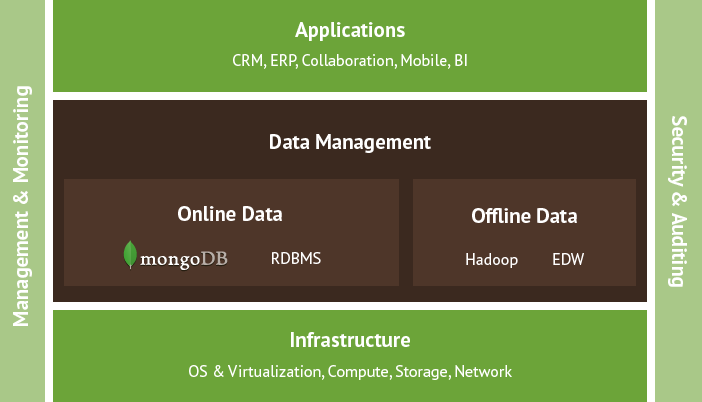
\includegraphics[scale=0.5]{mongodb_stack.png}
				\caption{mongodb stack}
			\end{center}
		\end{figure}
				
		\subsection{Introduction to MongoLab}
		MongoLab is a fully-managed cloud database service featuring highly-available MongoDB databases, automated backups, web-based tools, 24/7 monitoring, and expert support. Since its inception in 2011, MongoLab has grown like wildfire and now manages tens of thousands of databases across five major cloud providers in 13 datacenters worldwide.
		
		MongoLab help to connect to your database using standard MongoDB drivers in the language of your choice or use MongoLab's JSON-based REST API. It keeps your database close to your app server! MongoLab provides MongoDB hosting on all the major cloud platforms — Amazon, Google, Joyent, Rackspace, and Windows Azure — and has partnered with all of the major Platform-as-a-Service providers to enable seamless integration with the application tier.
	
	\section{Some UI Widget libraries}
		\subsection{Angular Bootstrap}
		Angular Bootstrap is Bootstrap components written in pure AngularJS which provide directive for using Twitter Bootstrap 's components and go along with AngularJS. They re-write some of Twitter Bootstrap 's components like accordion, drop-down, Modal, buttons into AngularJS 's directive for easier use and integration.
		\subsection{JqueryUI}
		Query UI is a curated set of user interface interactions, effects, widgets, and themes built on top of the jQuery JavaScript Library. It provides abstractions for low-level interaction and animation, advanced effects and high-level, themeable widgets, built on top of the jQuery JavaScript library, that can be used to build interactive web applications. 
		\subsection{Semantic-UI}
		Semantic-UI is the vocabulary of the web.Semantic empowers designers and developers by creating a language for sharing UI. It provides various kinds of widgets and components with modern design and effects.
	\section{HTML5}
	HTML5 aims to make HTML more useful for creating web applications as well as semantically marked up documents, is not yet a formal Recommendation as of this writing, however, it is beginning to gain browser support and is already being used for web and mobile application development.HTML5 offers new features (elements, attributes, event handlers, and APIs) for easier web application development and more sophisticated form handling. There are also new semantic elements for marking up page content. Most of the purely presentational or poorly supported elements and attributes in HTML 4.01 have been dropped from HTML5, however, a few have been redefined or reinstated.
	
	\section{CSS3}
	CSS (Cascading Style Sheets) consist of a group of formatting rules that you use to control the layout and appearance of the content on a web page. One really great feature of CSS is that you can store all the CSS rules in one document and keep that document separate from the HTML content and link the two together. Then, when you make a change to the CSS that change is instantly and automatically updated on all the HTML files. Another great feature is that it "cleans up" the appearance of the code on web pages. In addition it will speed up browser loading times.
\chapter{BUILDING AN APPLICATION USING SELECTED TECHNOLOGIES}
\textsl{The story in this chapter is about how all the state of the art technologies are integrated and utilized in every single piece of the application. Besides, All features are presented accordingly }
	\newpage 
	
	\section{Features}
			At first sight, the application consists of 4 main parts: Palettes, Canvas, Menu \& toolbar and sidebar as in figure ~\ref{interface}. Therefore, all the features can also be  divided into 4 different groups and will be described in details. Generally, the user can see all the shapes displayed based on category in the palettes on the left and drag into the canvas on the right. The user also interact with the diagram directly as well as see more information about a selected node in the sidebar. There are also menu and toolbar for the user to have many more options.
			\begin{figure}[ht]
				\begin{center}
					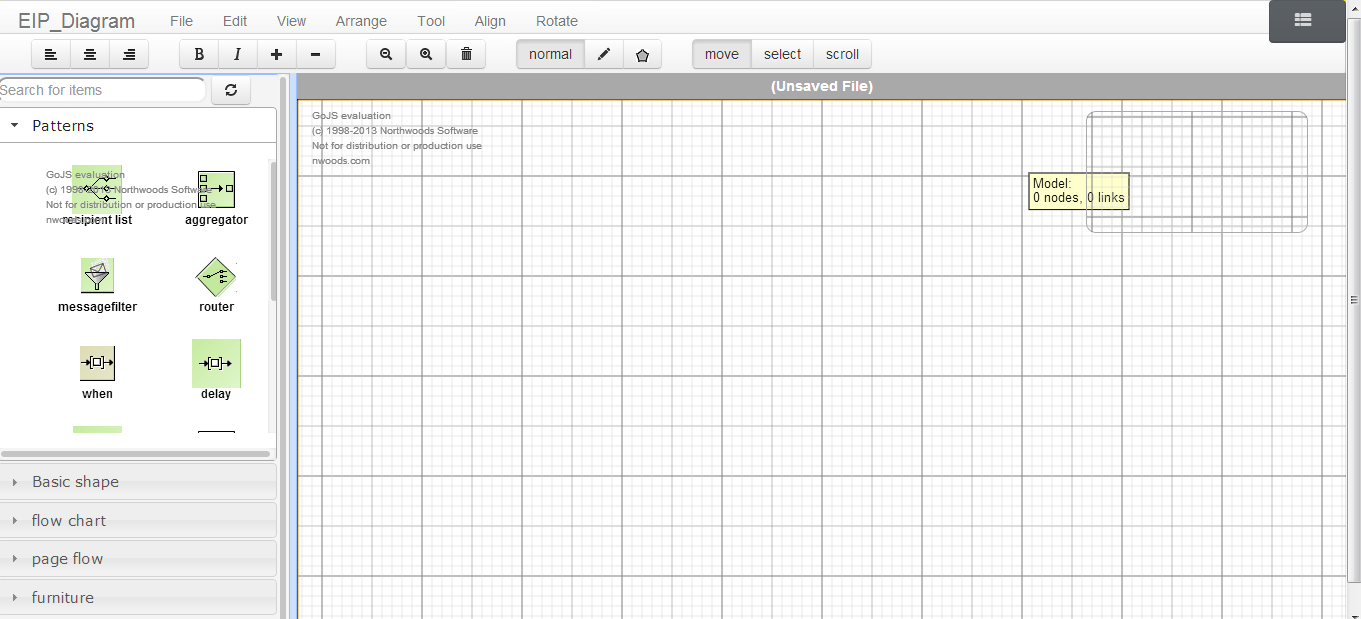
\includegraphics[scale=0.5]{interface.png}
					\caption{application 's interface}
					\label{interface}
				\end{center}
			\end{figure}
			
		\subsection{Palettes \& search}
		As in figure ~\ref{interface} The palettes are on the left of the application separated with the canvas by a splitter with can be handled to change the size of the palettes. Besides, many types of shapes are sorted by category, users can open the section with suitable category to see all the shapes. Moreover, there is a search box on top of the palettes. Users can find shapes by names or description and Enter to add that shape to the canvas as in figure ~\ref{search}
		\begin{figure}[ht]
				\begin{center}
					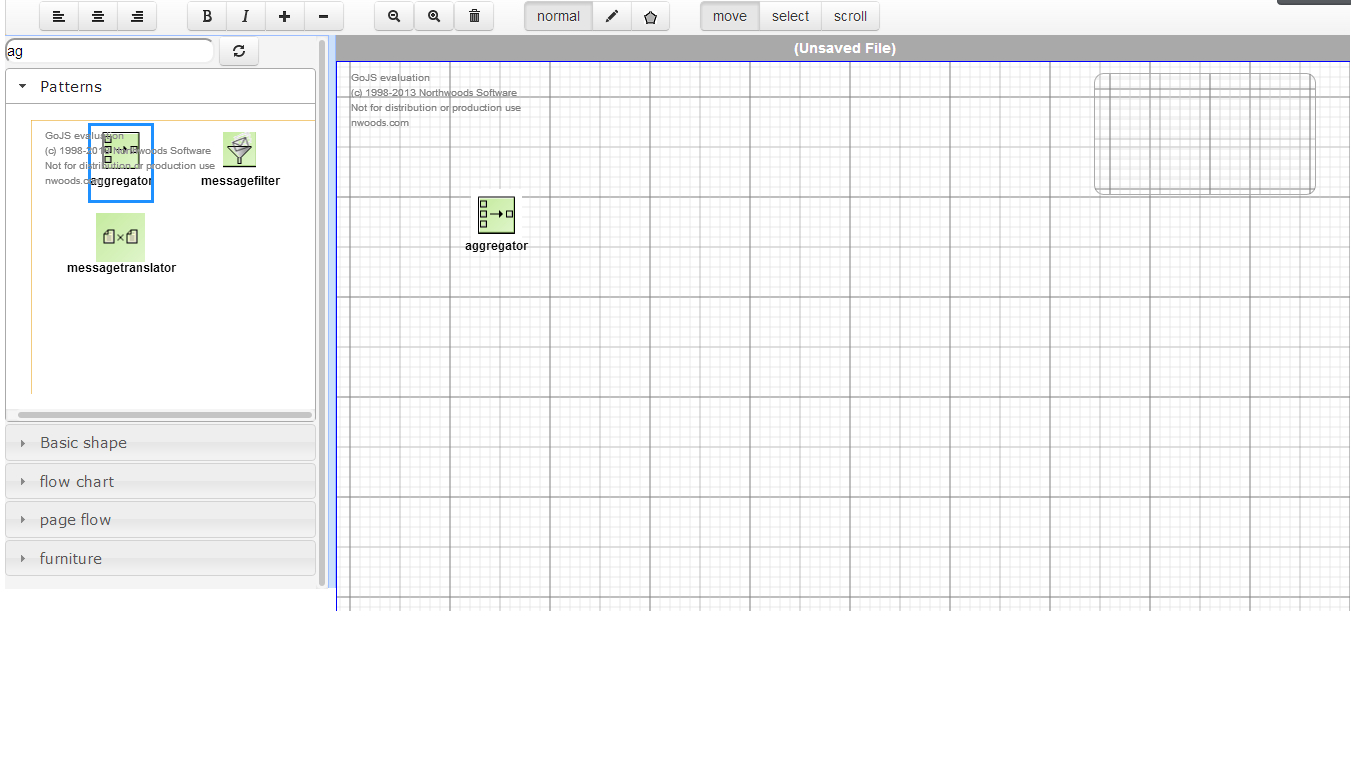
\includegraphics[scale=0.5]{search.png}
					\caption{Search function}
					\label{search}
				\end{center}
			\end{figure}
		
			
		\subsection{Interactive Diagram}
			\subsubsection{Double-click create}
				Doubld-click create cuts down several actions in traditional diagram software to 1 click action. That is much faster drawing! Add the next shape similar to the selected one immediately to the canvas with 1 double-click.
			\subsubsection{Context menu}	
				The context menu shows up by a single right-click base on what the user selected( node, link or background).
			\begin{figure}[ht]
				\begin{center}
					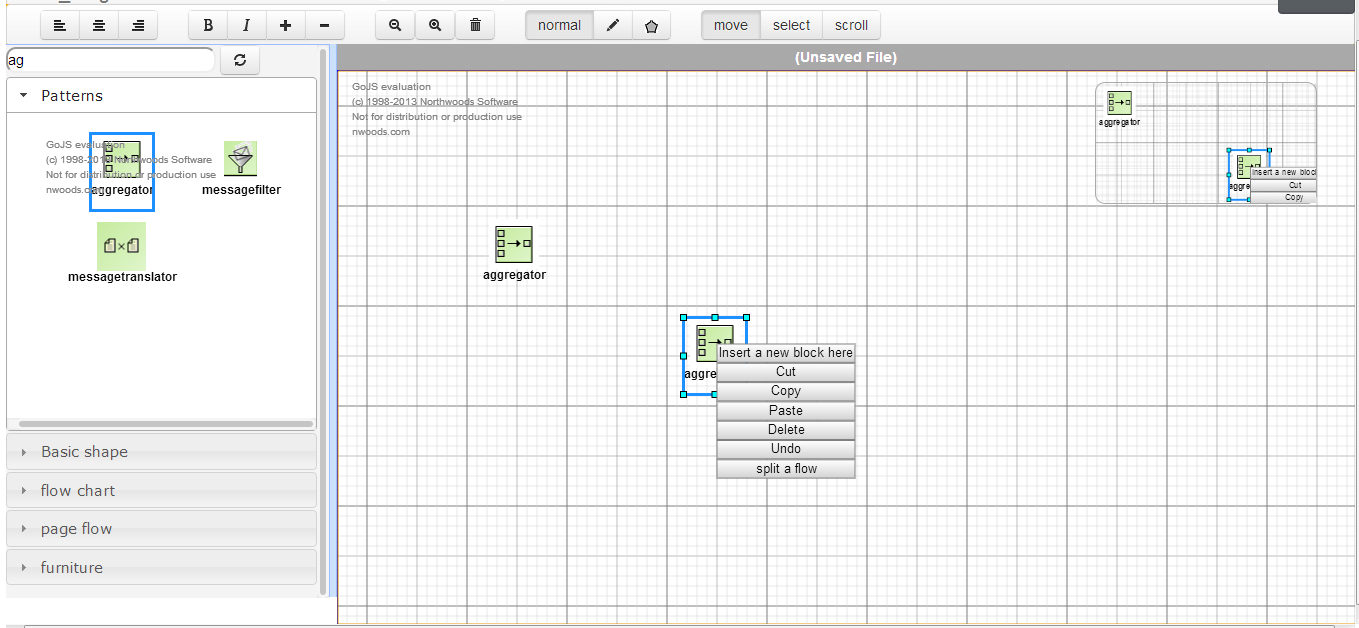
\includegraphics[scale=0.5]{contextmenu.png}
					\caption{context menu}
					\label{contextmenu}
				\end{center}
			\end{figure}
			\subsubsection{Connection}
				connecting object by mousing down on a port, move (drag) to nearby an input port, and then mouse-up to complete the link. The second way is to drag the node close in range and they will automatically connected. They will be connected by the whole node instead of a single port. By default the user may not draw more than one link in the same direction between any pair of ports, nor may the user draw a link connecting a node with itself.
			\subsubsection{Aligned, sized and grouped}
			Users can align a set of selected nodes, resize one or multiple nodes, and grouping one or many nodes. Adding more node to the group just by dragging.
				
		\subsection{Sidebar}
			The user can view information of a single selected node by open the sidebar as in figure ~\ref{sidebar}. They can view the type, width, height, position and change color of that node as in figure ~\ref{sidebarcolor}
			\begin{figure}[ht]
				\begin{center}
					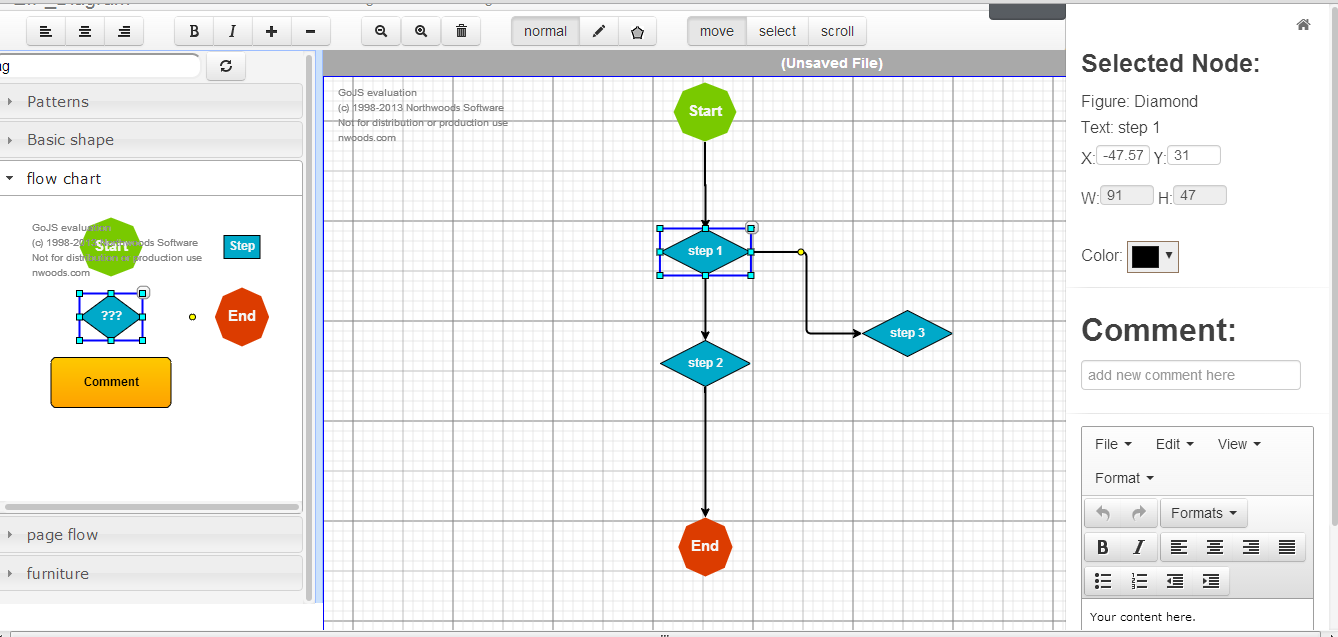
\includegraphics[scale=0.5]{sidebar.png}
					\caption{sidebar}
					\label{sidebar}
				\end{center}
			\end{figure}
			
			\begin{figure}[ht]
				\begin{center}
					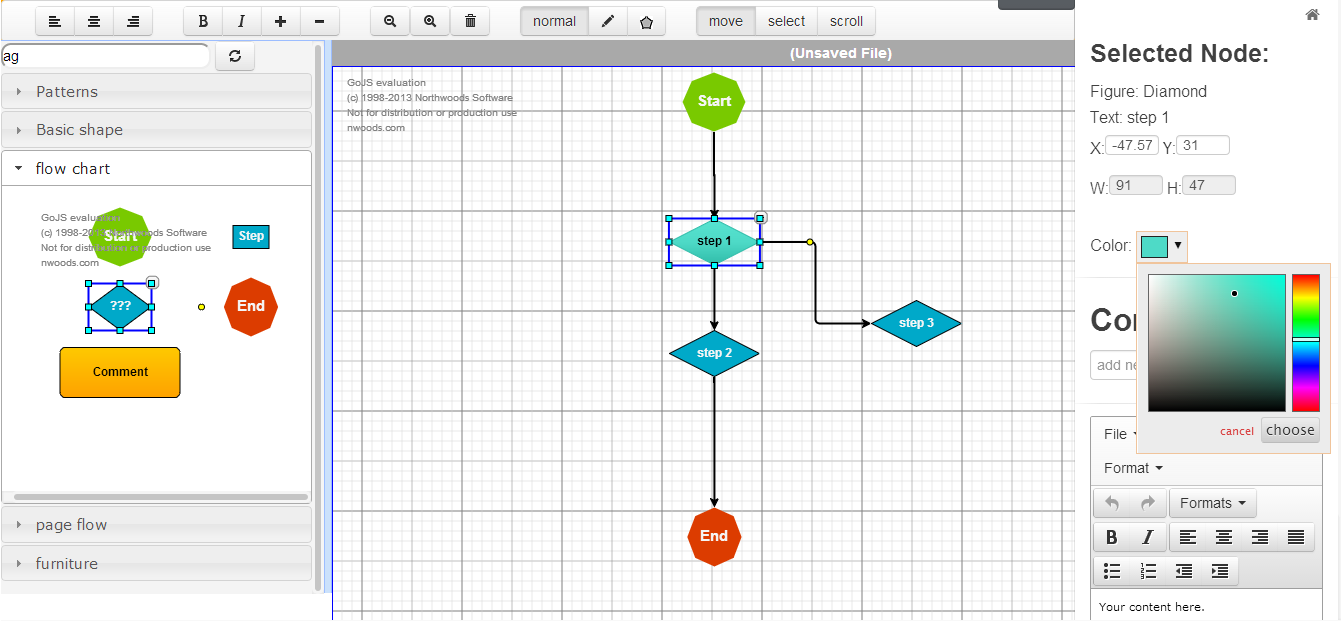
\includegraphics[scale=0.5]{sidebarcolor.png}
					\caption{change color of a node in sidebar}
					\label{sidebarcolor}
				\end{center}
			\end{figure}
		\subsection{Menu \& Toolbar}
			There are several categories on the Menu such as : file, Edit, View, Arrange, Tool, Align, Rotate with corresponding functions. On the toolbar there are some buttons for zooming, Change size of the node, text manipulation, copy, paste, delete
	\section{Database}
		MongoLab is a fully-managed cloud database service featuring highly-available MongoDB database. It's a NoSQL database which provides a mechanism for storage and retrieval of data that is modeled in means other than the tabular relations used in relational databases.
		In mongolab, documents and collections are used instead of tables and rows. This application uses two collections. They are Node (all the shape storage) and template ( for templates storage).
	\section{Front-end technologies}
		\subsection{Angular Bootstrap}
			In this application, buttons, font and menu are the widget that used from Bootstrap. This library also provide a set of glyph icon that is used in the toolbar.
		\subsection{JqueryUI}
			JqueryUI 's widgets are also integrated in this application. The palettes are made by using accordion component of this library. Besides, the splitter is also based on Jquery library that help to make nice animation.
		\subsection{Semantic-UI}
			The sidebar is a great widget using from semantic-ui library. It is a menu hidden beside page content and when activated it floats over the content of the page. It makes the theme clean and delicate with smooth animation.
	\section{Back-end technologies}

		\subsection{AngularJS}
			\subsubsection{application 's structure}
			The first thing AngularJS brought to the application is the structure. It should be clear already that Angular applications are structured very differently than similar applications were in the past.It has the services layer like in figure ~\ref{AngularStructure}, which is like a giant application brain that handles all of the state coordination, data persistence and the business logic. The angular controllers are like mini brains, less capable and are used to set up the initial state of the \$scope object or add behavior to the \$scope object. Templates and directives are like sensors and speech, which are responsible for displaying or "speaking" data to the user, and to take in outside information (like user events or data) and pass it to the controller. The application folders are also organized as in figure ~\ref{Angularfolder}.
		
		\begin{figure}
			\begin{center}
				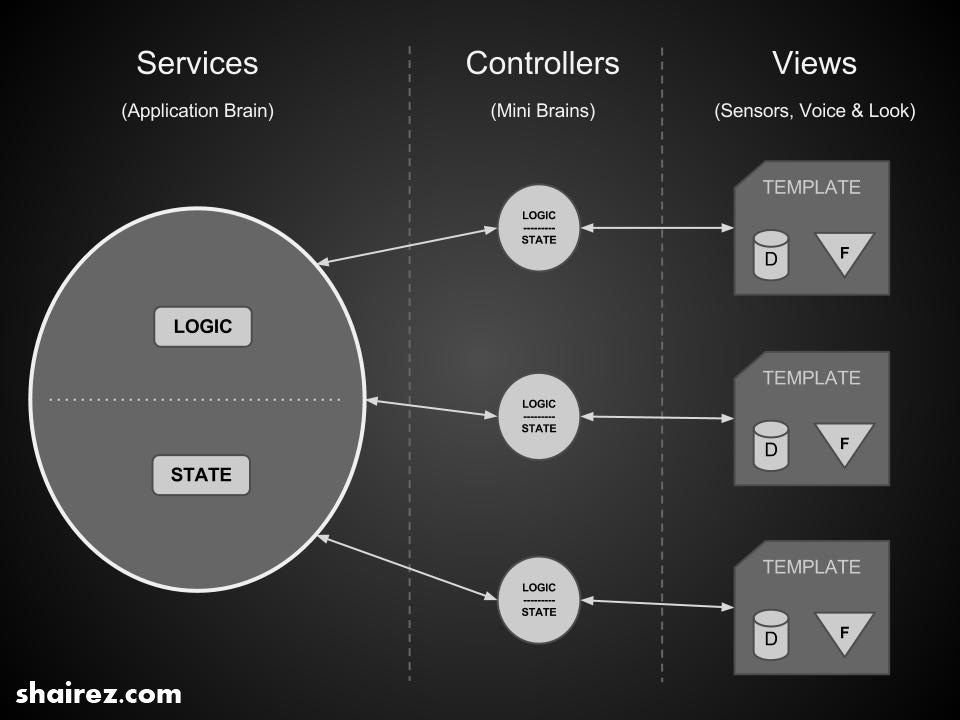
\includegraphics[scale=0.5]{angularArchitect.png}
				\caption{Angular application 's structure}
				\label{AngularStructure}
			\end{center}
		\end{figure}
		
		\begin{figure}
			\begin{center}
				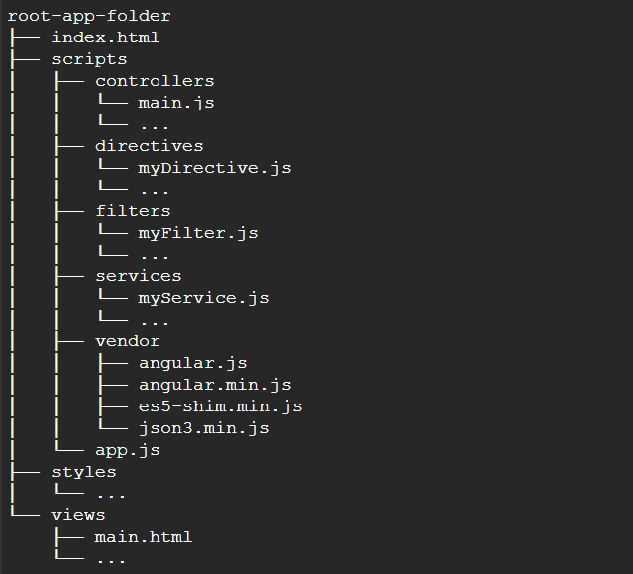
\includegraphics[scale=0.5]{angular_organize.png}
				\caption{Angular application 's folder organization}
				\label{Angularfolder}
			\end{center}
		\end{figure}

			\subsubsection{MVC}
			\subsubsection{Data Binding}
			Before AJAX single-page apps were common, platforms like Rails, PHP, or JSP helped us create the user interface (UI) by merging strings of HTML with data before sending it to the users to display it. Here with data binding i just declare which parts of the UI map to which JavaScript properties and have them sync automatically. It works great with MVC to eliminate code when writing view and model. Most of the work in moving data from one to the other just happens automatically. From now on the view will be automatically updated when the model changed . how great is this?
			\subsubsection{Changing the DOM with Directives}
			Directives extend HTML syntax, and are the way to associate behavior and DOM transformations with custom elements and attributes. Through them, it's very easy to create reusable UI components, configure the application, and do almost anything else ones can imagine wanting to do in the UI template. Writing apps with the built-in directives that come with Angular, but someteims, it's likely to run into situations where we want to write our own. It’s time to break into directives when dealing with browser events or modify the DOM in a way that isn’t already supported by the built-in directives. This code belongs in a directive that you write, and not in a controller, service, or any other place in your app.
			From now on instead of dealing with such long html code like this 
			\begin{verbatim}
			<div class="dropdown">
  <!-- Link or button to toggle dropdown -->
  <ul class="dropdown-menu" role="menu" aria-labelledby="dLabel">
    <li><a tabindex="-1" href="#">Action</a></li>
    <li><a tabindex="-1" href="#">Another action</a></li>
    <li><a tabindex="-1" href="#">Something else here</a></li>
    <li class="divider"></li>
    <li><a tabindex="-1" href="#">Separated link</a></li>
  </ul>
</div>
			\end{verbatim}
			we totally can write like this: 
			\begin{verbatim}
			<div dropdown-menu></div>
			\end{verbatim}
				Angular supports the Model View Controller style of application design. Though it has a lot of flexibility in designing an Angular application, a brief description of what MVC in figure ~\ref{MVC} can bring into this :
				\begin{itemize}
\item A model containing data that represents the current state of the application.
\item Views that display this data.
\item Controllers that manage the relationship between models and views
  				\end{itemize}
		\begin{figure}
			\begin{center}
				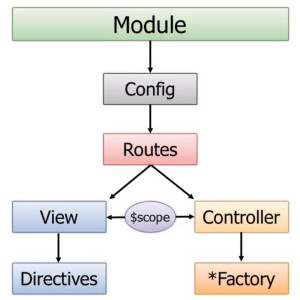
\includegraphics[scale=0.5]{angularmvc.png}
				\caption{MVC structure in Angular}
				\label{MVC}
			\end{center}
		\end{figure}
		

		\subsection{GoJS}
		
\chapter{DISCUSSION \& CONCLUSION}
	\textsl{In this chapter, discussion about all the explored technologies and evaluation about the application has just been built using and integrating such technologies. Besides, i will discuss further about the future work to improve performance as well as adding more features and improve code organization}
	\newpage 
	
	\section{Discussions of key technologies and concepts}
		\subsection{Front-end}
			This application uses some libraries that support and provide very beautiful and delicate widget such as accordion and splitter of JqueryUI, font, theme, color, menu of Twitter Bootstrap, Sidebar and modal of semantic-UI. They have very specific advantages that each library provide a nice set of Widgets and easily to integrate with other libraries. The combination of all these libraries gives the application a very delicate and nice look. Without such widgets, create an nice application takes a lot more times and effort and may cause errors.
		
		\subsection{Back-end}
			\subsubsection{AngularJS}
				AngularJS is an open-source JavaScript framework, maintained by Google, that assists with running single-page applications. Its goal is to augment browser-based applications with model–view–controller (MVC) capability, in an effort to make both development and testing easier. It give the RIA a nice structure with using many software enginering concepts like dependencies injection ,separation of concern and Inversion of control. 
				Utilizing such advantages, this application use Angular.js to structure and support the development.However, i cannot utilize all the advantages of angular like testing and some other services.
 			\subsubsection{GoJs}
 				GoJS is a feature-rich JavaScript library for implementing interactive diagrams across modern browsers and platforms. GoJS makes constructing diagrams of complex Nodes, Links, and Groups easy with customizable templates and layouts. GoJS offers many advanced features for user interactivity such as drag-and-drop, copy-and-paste, transactional state and undo management, palettes, overviews, data-bound models, event handlers, and an extensible tool system for custom operations.
 				However, this library lack support of UML component and sometimes there are still several errors happen.
		
		\subsection{Integration into one single RIA}
			It is such a nice work of integrating many frameworks and libraries together into one single RIA. This means this RIA is a combination of all the advantages of all the technologies which has been used. However, before the integration , a serious survey need to be conducted to choose such libraries that work together.
		
		\subsection{Software engineering concepts in RIA development}
			Two important software engineering concepts used in this RIA is Dependencies injection(DI) and Separation of concern. DI help the Reduction of boilerplate code – which is included in many places without any alteration and the programmers have to write more code to do minimum jobs in the application objects since all work to initialize or set up dependencies is handled by a provider component. Separation of Concerns (SoC) is a standard practice of dividing up major components of an application and segregating them from the rest of the application. There are many different ways to accomplish SoC and one of them is to utilize the magic of Dependency Injection (DI). SoC via DI is the practice of splitting up the application into components, and then resolving any dependencies those components have on other components through the use of injection.
			
	\section{Discussion of demo application}
		\subsection{Features and benefits}
			This RIA support design interactive diagram and collaboration with others.
		\subsection{Comparisons with other online diagram editors}
			There are some other diagram tool online such as draw.io, creately.com, griffy.com built by some big companies with stunning features. This application somehow can also provide similar features.
		\subsection{Drawbacks}
			Due to lack of experience and this is a one-person thesis so the scope is not big and the features cannot be compared with other tools built by large companies.
	\section{Future works and Conclusions}
		I have explore and apply many technology into an RIA development. I also present in-details about each technologies as well as the feature of this application. In the future, this application need to improve more about features as well as how to organize the function.


\begin{thebibliography}{99}
\bibitem{survey}{ "Surveying the digital future" UCLA Internet Report, http://www.digitalcenter.org/pdf/InternetReportYearThree.pdf}

\bibitem{Gvu} {“Gvu 10th www user survey,” GVU, http://www.cc.gatech.edu/gvu/user\_surveys/survey-1998-10/}

\bibitem{Center} “Center for the digital future: 2008 digital future report,” 2009. University of Southern California (USC) Annenberg School, C.F.T.D.F.

\bibitem{Internet} {L. Rainee, “Internet, broadband and cellphone statistics,” 2010. http://www.pewinternet.org/Reports/2010/Internet-broadband-and-cell-phone-statistics.aspx.}

\bibitem{Online} P. R. Center, “Online activities,” http://www.pewinternet.org/StaticPages/Trend-Data/Online-Activites-Total.aspx.

\bibitem{RIA} "Rich Internet application " http://en.wikipedia.org/wiki/Rich\_Internet\_application

\bibitem{WebApp} "Web Application" http://en.wikipedia.org/wiki/Web\_application

\bibitem{Real} Franz Josef Grüneberger , "REAL-TIME COLLABORATION SUPPORT FOR JAVASCRIPT FRAMEWORKS"

\bibitem{MT08} Tommi Mikkonen and Antero Taivalsaari. Web Applications Spaghetti Code for the 21st Century. In SERA, pages 319–328, 2008.

\bibitem{Ree79b} Trygve M. H. Reenskaug. Models - Views - Controllers. http://heim.ifi.uio.
no/~trygver/1979/mvc-2/1979-12-MVC.pdf, December 1979.

\bibitem{Ree79a} Trygve M. H. Reenskaug. Thing-Model-View-Editor - an Example from a Planningsys-tem. http://heim.ifi.uio.no/~trygver/1979/mvc-1/1979-05-MVC.
pdf, 1979.

\bibitem{BL12} Tim Berners-Lee. WorldWideWeb, the first Web Client. http://www.w3.org/People/Berners-Lee/WorldWideWeb.html, 2012.

\bibitem{TM11}Antero Taivalsaari and Tommi Mikkonen. The Web as an Application Platform: The Saga Continues. In EUROMICRO-SEAA, pages 170–174, 2011.

\bibitem{Gar05} Jesse James Garrett. AJAX: A New Approach to Web Applications. http://www.adaptivepath.com/ideas/ajax-new-approach-web-applications, 2005.
\end{thebibliography}



\end{document}
